%%%%%%%%%%%%%%%%%%%%%%%%%%%%%%%%%%%%%%%%%
% kaobook
% LaTeX Template
% Version 1.3 (December 9, 2021)
%
% This template originates from:
% https://www.LaTeXTemplates.com
%
% For the latest template development version and to make contributions:
% https://github.com/fmarotta/kaobook
%
% Authors:
% Federico Marotta (federicomarotta@mail.com)
% Based on the doctoral thesis of Ken Arroyo Ohori (https://3d.bk.tudelft.nl/ken/en)
% and on the Tufte-LaTeX class.
% Modified for LaTeX Templates by Vel (vel@latextemplates.com)
%
% License:
% CC0 1.0 Universal (see included MANIFEST.md file)
%
%%%%%%%%%%%%%%%%%%%%%%%%%%%%%%%%%%%%%%%%%

%----------------------------------------------------------------------------------------
%	PACKAGES AND OTHER DOCUMENT CONFIGURATIONS
%----------------------------------------------------------------------------------------

\documentclass[
	a4paper, % Page size
	fontsize=10pt, % Base font size
	twoside=true, % Use different layouts for even and odd pages (in particular, if twoside=true, the margin column will be always on the outside)
	%open=any, % If twoside=true, uncomment this to force new chapters to start on any page, not only on right (odd) pages
	%chapterentrydots=true, % Uncomment to output dots from the chapter name to the page number in the table of contents
	numbers=noenddot, % Comment to output dots after chapter numbers; the most common values for this option are: enddot, noenddot and auto (see the KOMAScript documentation for an in-depth explanation)
]{kaobook}

\usepackage[utf8]{inputenc}
\usepackage[italian]{babel}
\usepackage[T1]{fontenc}

\usepackage{algorithm}
\usepackage{algpseudocode}
\usepackage{tabu}
\usepackage{soul}

% Load packages for testing
\usepackage{blindtext}
%\usepackage{showframe} % Uncomment to show boxes around the text area, margin, header and footer
%\usepackage{showlabels} % Uncomment to output the content of \label commands to the document where they are used

% Load the bibliography package
%\usepackage{kaobiblio}
%\addbibresource{main.bib} % Bibliography file

% Load mathematical packages for theorems and related environments
\usepackage[framed=true]{kaotheorems}

% Load the package for hyperreferences
\usepackage{kaorefs}

\makeindex[columns=3, title=Alphabetical Index, intoc] % Make LaTeX produce the files required to compile the index

\makeglossaries % Make LaTeX produce the files required to compile the glossary
 % Include the glossary definitions

\makenomenclature % Make LaTeX produce the files required to compile the nomenclature

% Reset sidenote counter at chapters
%\counterwithin*{sidenote}{chapter}

%----------------------------------------------------------------------------------------

\begin{document}

%----------------------------------------------------------------------------------------
%	BOOK INFORMATION
%----------------------------------------------------------------------------------------


\title[{\normalfont\texttt{kaobook}} class]{Network Security}
\subtitle{Anno 2022-2023}


\date{\today}

%----------------------------------------------------------------------------------------

\frontmatter % Denotes the start of the pre-document content, uses roman numerals

%----------------------------------------------------------------------------------------
%	OPENING PAGE
%----------------------------------------------------------------------------------------

%\makeatletter
%\extratitle{
%	% In the title page, the title is vspaced by 9.5\baselineskip
%	\vspace*{9\baselineskip}
%	\vspace*{\parskip}
%	\begin{center}
%		% In the title page, \huge is set after the komafont for title
%		\usekomafont{title}\huge\@title
%	\end{center}
%}
%\makeatother


%----------------------------------------------------------------------------------------
%	DEDICATION
%----------------------------------------------------------------------------------------

\dedication{
	I procioni sono meglio dei panda rossi.\\
	%\flushright -- 
}

%----------------------------------------------------------------------------------------
%	OUTPUT TITLE PAGE AND PREVIOUS
%----------------------------------------------------------------------------------------

% Note that \maketitle outputs the pages before here

\maketitle

\tableofcontents % Output the table of contents


%----------------------------------------------------------------------------------------
%	MAIN BODY
%----------------------------------------------------------------------------------------

\mainmatter % Denotes the start of the main document content, resets page numbering and uses arabic numbers
\setchapterstyle{kao} % Choose the default chapter heading style

\setchapterpreamble[u]{\margintoc}
\chapter{Introduzione}
\labch{chapter1}

La sicurezza informatica è l'insieme di strumenti, politiche, sicurezza concetti, misure di sicurezza, linee guida, gestione dei rischi approcci, azioni, formazione, best practice, garanzia e tecnologie che possono essere utilizzate per proteggere il cyberspazio ambiente, organizzazione e risorse degli utenti. Le risorse dell'organizzazione e degli utenti includono dispositivi informatici connessi, personale, infrastrutture, applicazioni, servizi, sistemi di telecomunicazione e la totalità delle informazioni trasmesse e / o memorizzate nell'ambiente del cyberspazio.

La sicurezza informatica si impegna a garantire il raggiungimento e Mantenimento delle proprietà di sicurezza dell'organizzazione e le risorse degli utenti contro i rischi per la sicurezza rilevanti nel ambiente del cyberspazio. Gli obiettivi generali di sicurezza comprendono quanto segue: disponibilità; integrità, che può includere l'autenticità dei dati e il non ripudio; e riservatezza
\setchapterpreamble[u]{\margintoc}
\chapter{Distribuzione e gestione delle chiavi crittografiche}
\labch{chapter3}

La sicurezza delle chiavi crittografiche dipende dal modo con cui sono protette. Il managment di queste chiavi comprende la loro generazione, creazione, protezione, salvataggio, scambio, sostituzione e uso. Permette inoltre di restringere l'accesso alle chiavi e monitorarne/registrarne ogni accesso, uso e contesto.
Il sistema di gestione delle chiavi comprende anche le chiavi dei server, le procedure utente e i protocolli.
La sicurezza del sistema crittografico dipende anche da una gestione corretta delle chiavi.

Tecnica di distribuzione delle chiavi: 
\begin{itemize}
    \item Riguarda la consegna di una chiave a due parti che vogliono scambiarsi dati senza che terzi vedano la chiave;
	\item Affichè la crittografia simmetrica funziona, le due parti devono condividere la stessa chiave, che deve essere protetta da accessi non autorizzati;
	\item È desiderabile cambiare frequentemente la chiave per limitare la quantità di dati che verrebbero compromessi se un attaccante ottenesse la chiave.
\end{itemize}

Possibili modi per la distribuzione di chiavi simmetriche (figura \ref{fig:3-1}):
\begin{itemize}
    \item A sceglie una chiave e la consegna fisicamente a B;
	\item Un terzo sceglie la chiave e la consegna fisicamente ad A e B;
	\item Se A e B hanno condiviso una chiave recentemente, un terzo può scegliere una nuova chiave e inviarla, cifrata con la vecchia chiave, ad A e B;
    \item Se A e B hanno una connessione cifrata con C, C può inviare la chiave sul canale cifrato ad A e B.
\end{itemize}

In riferimento allo schema:
\begin{itemize}
    \item Key Transaltion Center: riceve una chiave da un'entità A cifrata con una chiave simmetrica condivisa tra A e KTC, la decifra e la invia all'entità B cifrata con la chiave simmetrica condivisa tra B e KTC. È considerato trusted.
    \item Kma: chiave simmetrica condivisa tra A e KTC. Esiste quindi un canale sicuro tra i due.
\end{itemize}

\begin{figure}
    \centering
    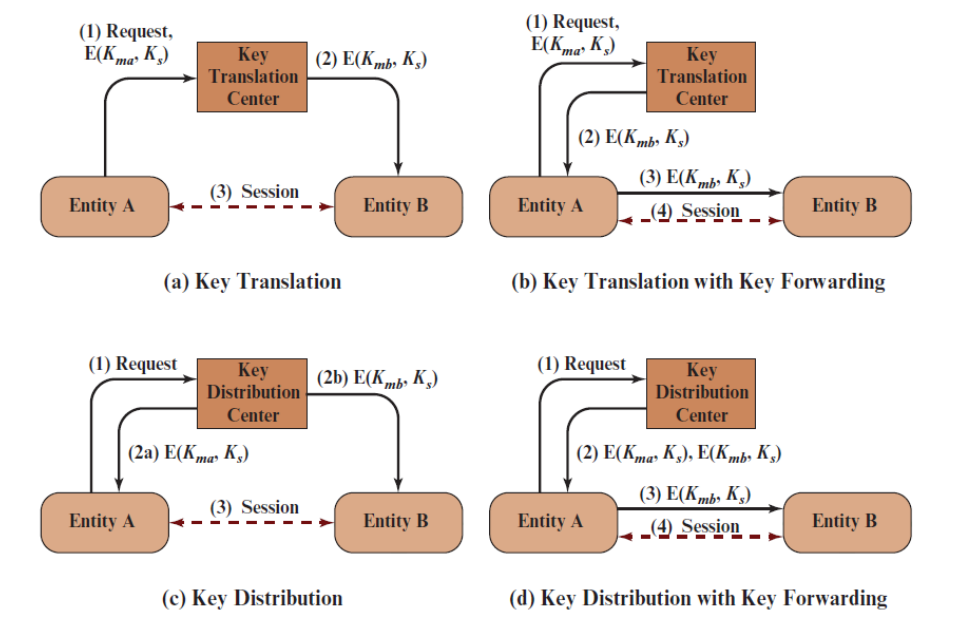
\includegraphics[width=1\textwidth]{images/chapter3/3-1.png}
    \caption{Possibili distribuzioni della chiave.}
    \label{fig:3-1}
\end{figure}

Generalmente la chiave simmetrica scambiata all'inizio della comunicazione viene considerata come master key e usata per generare una serie di sottochiavi simmetriche. Più in basso nella gerarchia sono le sottochiavi, più la loro durata diminuisce e il loro uso aumenta.

\paragraph{Semplice scambio di chiavi usando chiavi pubbliche} A invia la propria chiave pubblica e identità a B. B risponde inviando la chiave di sessione cifrata con la chiave pubblica di A (figura \ref{fig:3-2}). 

\begin{figure}
    \centering
    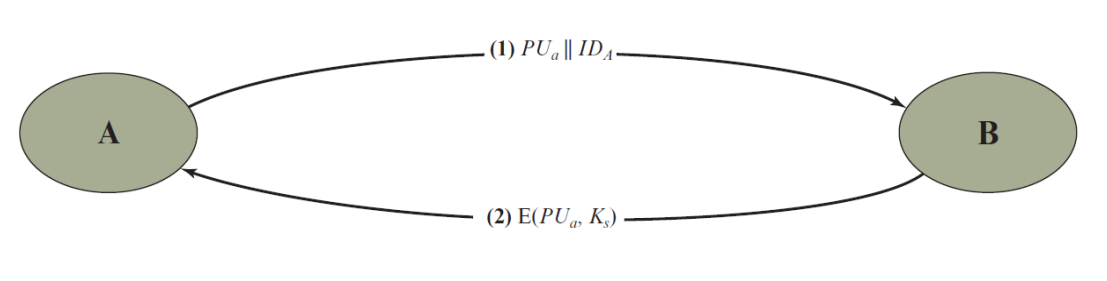
\includegraphics[width=1\textwidth]{images/chapter3/3-2.png}
    \caption{Scambio semplice.}
    \label{fig:3-2}
\end{figure}

Questa soluzione è però debole ad un attacco man-in-the-middle: 
\begin{enumerate}
    \item C cattura il messaggio di A; 
	\item Sostituisce la chiave pubblica di A con la sua (lasciando inalterata l'identità);
	\item B codifica la chiave di sessione con la PU che crede sia di A e invia il messaggio;
	\item C cattura la risposta, decifra il messaggio, lo ricifra con la PU di A e glielo invia;
	\item A riceve la chiave e la comunicazione è stabilità;
	\item C può decifrare ora tutti i messaggi scambiati sul canale.
\end{enumerate}

\paragraph{Scambio di chiavi con chiavi pubbliche e nonce\sidenote{Nonce: stringa randomica che viene usata per verificare che un messaggio non sia stato modificato/sostituito (protegge anche dai replay attack). Se la risposta non contiene lo stesso nonce che ho inviato nella richiesta, allora la scarto.}} Lo scambio prevede una serie di passaggi (figura \ref{fig:3-3}):
\begin{itemize}
    \item A invia la propria identità e un nonce entrmbi cifrati con la PU di B; 
    \item B Invia il nonce generato da A e un proprio nonce cifrati con la PU di A;
    \item A invia il nonce ricevuto da B cifrato con la PU di B;
    \item A e B si sono ora autenticati l'un l'altro, quindi B invia la chiave di sessione cifrata con la propria chiave privata, il tutto cifrato con la chiave pubblica di B.
\end{itemize}

\begin{figure}
    \centering
    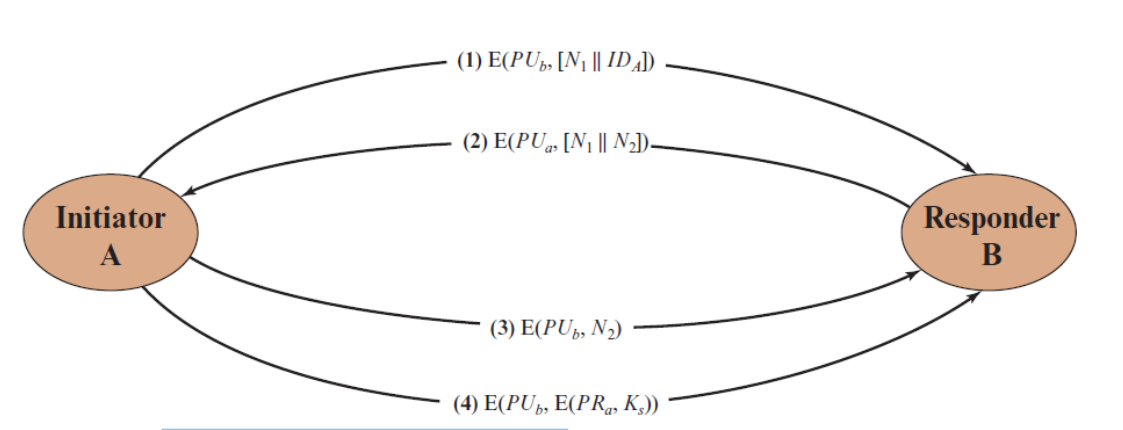
\includegraphics[width=1\textwidth]{images/chapter3/3-3.png}
    \caption{Scambio semplice.}
    \label{fig:3-3}
\end{figure}

Anche questo scambio è debole, in quanto C può mettersi in mezzo e far credere ad A e B, nei primi 3 passi, di star comunicando.

\section{Distribuzione delle chiavi pubbliche}

L'autority mantiene una directory con nome/certificato,chiave pubblica, che è facilmente accessibile.

Scenario di distribuzione (figura \ref{fig:3-4}):
\begin{enumerate}
    \item A richiede all'autority la chiave pubblica di B. Nel messaggio inserisce un timestamp;
	\item L'autority invia la chiave cifrata con la chiave pubblica dell'autority. Nel messaggio cifrato riporta il timestamp ricevuto da A;
	\item A invia la propria identità e un nonce a B;
	\item B richiede all'authority la chiave pubblica di A. Nel messaggio inserisce un timestamp;
	\item L'autority invia la chiave pubblica di A cifrata con la chiave privata dell'autority. Nel messaggio cifra anche il timestamp ricevuto;
	\item B invia, cifrati con la chiave pubblica di A, il nonce ricevuto da A e un nonce da lei generato;
	\item A invia a B il nonce ricevuto cifrato con la chiave pubblica di B.
\end{enumerate}

\begin{figure}
    \centering
    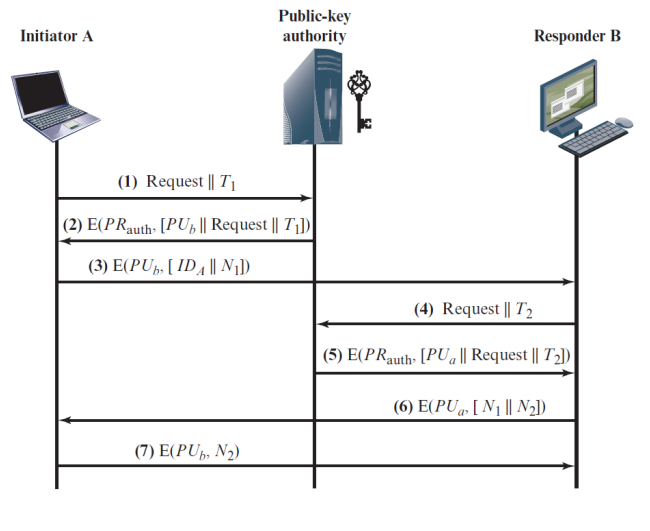
\includegraphics[width=1\textwidth]{images/chapter3/3-4.png}
    \caption{Scambio semplice.}
    \label{fig:3-4}
\end{figure}

Il certificato può essere ottenuto dalla Certification Autority o dall'utente.

\subsection{Certificati X.509}

Parte della serie X.500 che definisce un servizio di directory. Una directory può essere un serve o un insieme di server che mantengono un DB con info sugli utenti. 
Lo standard X.509 definisce un framework per la fornitura di servizi di autenticazione dalle directory dell'X.500 agli utenti (raccomanda RSA, non specifica l'algoritmo di hash da usare).

Uso del certificato:
\begin{itemize}
    \item Il certificato è "formato" da due parti: il certificato vero e proprio e il certificato firmato;
	\item Il certificato firmato non è altro che l'hash del certificato firmato con la chiave privata della CA;
	\item Un utente che vuole verificare il certificato passa all'algoritmo di verifica l'hash del certificato, il certificato firmato e la chiave pubblica della CA.
\end{itemize}

Un certificato si compone di:
\begin{itemize}
    \item Versione del certificato;
	\item Numero seriale del certificato all'interno della CA che l'ha rilasciato;
	\item Identificatore dell'algoritmo usato per la firma;
	\item Nome della CA;
	\item Periodo di validità:
	\item Nome dell'utente;
	\item Info culla chiave pubblica dell'utente;
	\item ID unico della CA;
	\item ID unico dell'utente;
	\item Estensioni;
	\item Firma (certificato firmato).
\end{itemize}

I certificati generati da una CA hanno le seguenti caratteristiche:
\begin{itemize}
    \item Ogni utente che ha accesso alla chiave pubblica della CA può verificare la chiave pubblica di un altro utente firmata dalla CA;
	\item Nessuno, eccetto la CA, può modificare un certificato senza essere individuato.
	\item Poiché i certificato non possono essere forgati, la directory in cui sono piazzati non richiede troppa sicurezza;
	\item Una volta che B è in possesso del certificato di A, sa che i messaggi cifrati con la chiave pubblica di A saranno al sicuro da intercettazione e che i messaggi firmati con la chiave privata di A saranno inforgiabili.
\end{itemize}

Catena di certificati: A vuole verificare il certificato di B, ma non conosce la chiave pubblica della CA di B. Se le due CA si sono scambiate le proprie chiavi (si sono certificate tra loro), A la può recuperare dalla directory della sua CA. In caso contrario, a partire dalle CA con cui la CA di A si è scambiata le chiavi, si procede a cercare la prima coppia di CA (una parente di A e una di B) che si sono certificate tra loro. Si costruisce quindi una catena di certificati. La catena ha la forma di un albero. Se un nodo, quindi CA, viene compromesso, allora anche il sottoalbero figlio viene considerato compromesso.

Revoca del certificato:
\begin{itemize}
    \item Ogni certificato contiene un periodo di validità, che solitamente viene sostituito prima della scadenza;
	\item Generalmente si tende a revocare un certificato prima della scadenza se:
	\begin{itemize}
	    \item La chiave privata dall'utente è compromessa;
		\item L'utente non è più certificato dalla CA;
		\item La CA è compromessa.
	\end{itemize}
	\item Ogni CA deve mantenere e rendere accessibile una lista dei certificati revocati non per scadenza.
\end{itemize}

\subsection{Certificati X.509 V3}

Include la possibilità di specificare estensioni (piuttosto che continuare ad aggiungere nuovi campi). Le estensioni possono riguardare:
\begin{enumerate}
    \item Info sulla chiave o sulla policy: copre info addizionali sull'utente e la CA, più indicatori sulle policy del certificato. Una policy sul certificato è un insieme nominato di regole che indica l'applicabilità del certificato a particolari comunità o classi di applicazioni con requisiti di sicurezza comuni. Contiene:
	\begin{itemize}
	    \item ID della chiave della CA;
		\item ID della chiave dell'utente;
		\item Uso della chiave (firma digitale, ripudio, crittografia delle chiavi, ecc.);
		\item Periodo di utilizzo della chiave privata;
		\item Policy del certificato;
		\item Mapping delle policy (consente a una CA di indicare altre CA equivalenti).
	\end{itemize}
		
	\item Attributi sulla CA o sull'utente: supportano nomi alternativi, in formati alternativi, per un soggetto del certificato o un emittente del certificato. Può contenere informazioni aggiuntive sul soggetto del certificato per aumentare la fiducia dell'utente del certificato che il soggetto del certificato sia una determinata persona o entità. I campi dell'estensione comprendono:
	\begin{itemize}
	    \item Nome alternativo del soggetto;
		\item Nome alternativo dell'emittente;
		\item Attributi sulla directory del soggetto.
	\end{itemize}
		
	\item Vincoli sul certificato: permettono di includere le specifiche di vincolo nei certificati emessi per CA da altre CA. I vincoli possono restringere le tipologie di certificati che possono essere emessi dalla CA soggetto o che possono verificarsi successivamente in una catena di certificazione. I campi sono:
	\begin{itemize}
	    \item Vincoli di base;
		\item Vincoli sui nomi;
		\item Vincoli sulle policy
	\end{itemize}
\end{enumerate}

Ogni estensione contiene: ID dell'estensione, indicatore di criticità, valore dell'estensione.

\subsection{Possibile scenario}
La RA ha il compito di raccogliere info su Bob per assicurarsi che sia chi dica di essere (\ref{fig:3-5}).

\begin{figure}
    \centering
    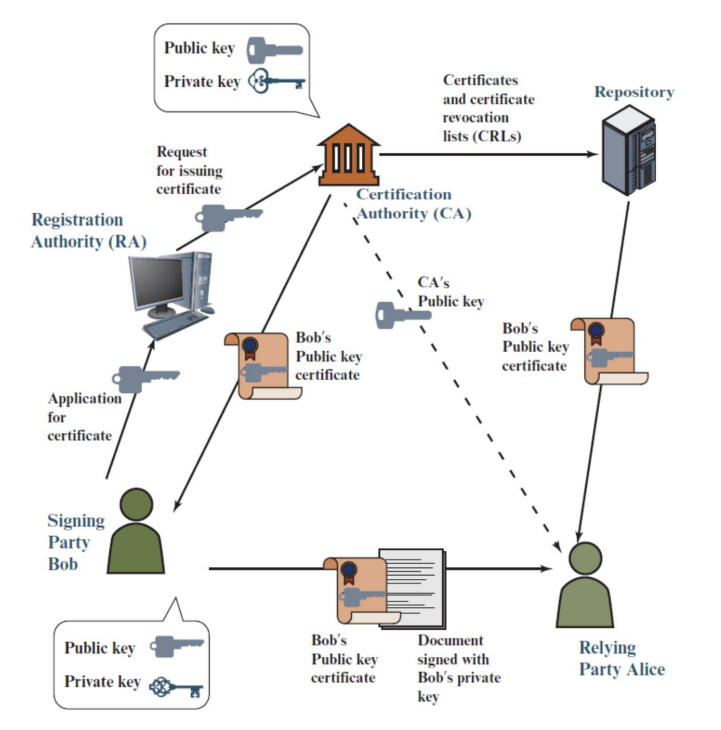
\includegraphics[width=1\textwidth]{images/chapter3/3-5.png}
    \caption{Scambio semplice.}
    \label{fig:3-5}
\end{figure}
\setchapterpreamble[u]{\margintoc}
\chapter{Autenticazione utente}
\labch{chapter4}

Autenticazione utente:
\begin{itemize}
    \item Processo per determinare se un utente o qualche applicazione o processo che agisce per conto di un utente è, in effetti, chi o cosa dichiara di essere;
	\item La tecnologia di autenticazione fornisce il controllo dell'accesso ai sistemi controllando se le credenziali di un utente corrispondono alle credenziali in un database di utenti autorizzati o in un server di autenticazione dati;
	\item L'autenticazione consente alle organizzazioni di proteggere le proprie reti consentendo solo agli utenti (o processi) autenticati di accedere alle risorse protette;
	\item L'autenticazione dell'utente è distinta dall'autenticazione del messaggio: l'autenticazione del messaggio è una procedura che consente alle parti comunicanti di verificare che il contenuto di un messaggio ricevuto non sia stato alterato e che la fonte sia autentica.
\end{itemize}

Principi dell'autenticazione:
\begin{itemize}
    \item \textbf{Identità digitale}: rappresentazione unica di un soggetto impegnato in una transazione online. Consiste in un attributo o insieme di attributi che descrivono in modo univoco un soggetto all'interno di un dato contesto di un servizio digitale, ma non identificano necessariamente in modo univoco il soggetto in tutti i contesti;
	\item \textbf{Prova dell'identità}: stabilisce che un soggetto è chi afferma di essere ad un determinato livello di certezza. Consiste nella raccolta delle info sull'utente e la creazione della sua identità (primo accesso);
	\item \textbf{Autenticazione digitale}: processo di determinazione della validità di uno o più autenticatori utilizzati per rivendicare un'identità digitale. La riuscita dell'autenticazione fornisce garanzie ragionevoli basate sul rischio che il soggetto che accede al servizio oggi è lo stesso del soggetto che ha precedentemente effettuato l'accesso al servizio (dal secondo accesso in poi).
\end{itemize}

Mezzi di autenticazione:
\begin{itemize}
    \item Qualcosa che si conosce;
	\item Qualcosa che si possiede;
	\item Qualcosa che si è o si fa;
\end{itemize}

\section{Autenticazione reciproca}
I protocolli che consentono alle parti comunicanti di soddisfarsi reciprocamente sull'identità dell'altro e di scambiare chiavi di sessione devono gestire due problematiche:
\begin{itemize}
    \item \textbf{Riservatezza}: info sull'identità e sulle chiavi di sessione devono essere scambiate in forma cifrata. Questo richiede la preventiva esistenza di chiavi segrete o pubbliche utilizzabili a tale scopo;
	\item \textbf{Tempestività}: importante a causa della minaccia di ripetizioni dei messaggi. I replay potrebbero permettere all'attaccante di:
	\begin{itemize}
	    \item Compromettere una chiave di sessione;
		\item Impersonare con successo l'altra parte;
		\item Interrompere le operazioni presentando alle parti messaggi che sembrano autentici ma non lo sono.
	\end{itemize}
\end{itemize}

Possibili replay attack:
\begin{itemize}
    \item L'attacco più semplice è quello in cui l'avversario copia semplicemente un messaggio e lo riproduce in seguito:
	\item Un avversario può riprodurre un messaggio con timestamp entro la finestra temporale valida;
	\item Un avversario può riprodurre un messaggio con timestamp entro la finestra temporale valida, ma in aggiunta, l'avversario sopprime il messaggio originale; quindi, la ripetizione non può essere rilevata;
	\item Un altro attacco prevede un replay all'indietro senza modifica ed è possibile se viene utilizzata la crittografia simmetrica e il mittente non può riconoscere facilmente la differenza tra messaggi inviati e messaggi ricevuti in base al contenuto (reflection attack).
\end{itemize}

Protezione dai replay attack:
\begin{itemize}
    \item Aggiungere un sequence number a ciascun messaggio utilizzato in uno scambio di autenticazione. Un nuovo messaggio viene accettato solo se il numero di sequenza è nell'ordine corretto. La difficoltà con questo approccio è che richiede a ciascuna parte di tenere traccia dell'ultimo numero di sequenza per ogni altra parte con cui ha avuto a che fare. Generalmente non è usato nell'autenticazione e nello scambio delle chiavi perché genera overhead;
	\item Aggiungere un timestamp. Richiede la sincronizzazione degli orologi tra i vari partecipanti. A accetta il messaggio solo se il timestamp rientra nel tempo di attesa accettato;
	\item Usare una challenge-response. A invia un nonce a B (challenge) e si aspetta che la risposta di B lo contenga (response).
\end{itemize}

\underline{Suppress Replay Attack}: Il protocollo di Denning richiede l'utilizzo di orologi sincronizzati in tutta la rete. È un vincolo rischioso in quanto gli orologi distribuiti possono non sincronizzarsi a causa di sabotaggi o guasti negli orologi stessi o nel meccanismo di sincronizzazione. Il problema si verifica quando l'orologio di un mittente è in anticipo rispetto all'orologio del destinatario: l'attaccante può intercettare il messaggio, catturarlo e rinviarlo quando il timestamp del messaggio è sincronizzato con l'orologio del ricevente.

Autenticazione remota dell'utente con chiave simmetrica:
\begin{itemize}
    \item È possibile utilizzare una gerarchia a due livelli di chiavi simmetriche per garantire la riservatezza per le comunicazioni in un ambiente distribuito;
	\item La strategia prevede l'uso di un centro di distribuzione delle chiavi affidabile (KDC);
	\item Ciascuna parte condivide una chiave segreta, nota come master key, con il KDC;
	\item Il KDC ha il compito di generare e distribuire le chiavi temporanee usate nella connessione. Le distribuzione delle chiavi temporanee viene protetta usando le master key.
\end{itemize}

\section{Kerberos}

Servizio di autenticazione sviluppato nell'ambito del Progetto Athena al MIT. Si basa sul concetto che non ci si può fidare di una workstation per identificare correttamente i suoi utenti per l'accesso ai servizi di rete:
\begin{itemize}
    \item Un utente può accedere a una determinata workstation e fingere di essere un altro utente che opera da quella workstation;
	\item Un utente può modificare l'indirizzo di rete di una workstation in modo che le richieste inviate dalla workstation modificata sembrino provenire dalla workstation rappresentata;
	\item Un utente può intercettare gli scambi e utilizzare un replay attack per accedere a un server o interrompere le operazioni.
\end{itemize}

Kerberos fornisce un server di autenticazione centralizzato la cui funzione consiste nell'autenticare gli utenti sui server e i server sugli utenti. Utilizza solo crittografia simmetrica (no chiavi pubbliche).

Requisiti:
\begin{itemize}
    \item Sicuro: un intercettatore sulla rete non dovrebbe essere in grado di ottenere le informazioni necessarie per impersonare un utente;
	\item Affidabile: dovrebbe essere altamente affidabile e dovrebbe impiegare un'architettura a server distribuiti con un sistema in grado di eseguire il backup di un altro;
	\item Trasparente: idealmente, l'utente non dovrebbe essere consapevole del fatto che l'autenticazione sta avvenendo oltre al requisito di immissione di una password;
	\item Scalabile: il sistema dovrebbe essere in grado di supportare un numero elevato di client e server.
\end{itemize}

\subsection{Kerberos v.4 (1988)}

Utilizza DES per fornire il servizio di autenticazione.

Componenti:
\begin{enumerate}
    \item Server di autenticazione (AS): conosce le password di tutti gli utenti e le archivia in modo centralizzato. Condivide una chiave univoca con ogni server;
	\item Ticket generale: creato una volta che l'AS accetta l'utente come autentico; contiene l'ID dell'utente e l'indirizzo di rete e l'ID del server-granting ticket (TGS). Il ticket è cifrato usando la chiave condivisa tra l'AS e quel TGS;
	\item Ticket-granting server (TGS): emette ticket specifici per permette all'utente di accedere ai servizi. Ogni volta che l'utente deve accedere ad un servizio, presenta al TGS il ticket generale ricevuto dall'AS. Il TGS verifica il ticket e genera un ticket specifico che l'utente userà per autenticarsi al server che gestisce il servizio/risorsa che ha richiesto.
\end{enumerate}
	
Problemi da tener presente nello scambio dei messaggi:
\begin{itemize}
    \item La durate del ticket generale può essere un problema:
	\begin{itemize}
	    \item Se la durata è molto breve (es. minuti), all'utente verrà ripetutamente richiesta una password (deve riautenticarsi con l'AS);
		\item Se la vita è lunga (ad esempio, ore), allora aumentano le possibilità di un replay attack.
	\end{itemize}
	\item Un servizio di rete (il TGS o un servizio applicativo) deve essere in grado di provare che la persona che utilizza un biglietto è la stessa persona a cui è stato emesso quel biglietto (utilizzare un autenticatore).
	\item Inoltre i server devono autenticarsi agli utenti (tramite un secondo autenticatore).
\end{itemize}

Scambio dei messaggi (figura \ref{fig:4-1}):
\begin{enumerate}
    \item Il client contatta l'AS per richiedere l'accesso al servizio del TGS;
	\begin{itemize}
	    \item Messaggio = [ID client, ID TGS, timestamp1]
	\end{itemize}
	\item L'AS invia il ticket generale al client. Il messaggio è cifrato con una chiave che l'AS deriva dalla password del client (che conosce). Ricevuto il messaggio il client calcolerà la chiave a partire dalla chiave passata dall'utente: 
	\begin{itemize}
	    \item Messaggio = [ID TGS, timestamp2, ticket generale]
		\item Ticket = [chiave di sessione per client e TGS, ID client, indirizzo client, ID TGS, timestamp2, tempo di vita del ticket]
		\begin{itemize}
		    \item Ticket cifrato con la chiave condivisa tra TGS e AS
		\end{itemize}
	\end{itemize}
	\item Il client contatta il TGS per richiedere l'accesso al servizio;
	\begin{itemize}
	    \item Messaggio = [ID client, ticket generale, autenticatore]
		\item Autenticatore = [ID client, indirizzo client, timestamp4]
	\end{itemize}
	\item Il TGS fornisce al client il ticket per accedere al server che gestisce il servizio;
	\begin{itemize}
	    \item Messaggio = [chiave di sessione generata dal TGS per la comunicazione tra client e server, ID client, timestamp4, ticket]
		\begin{itemize}
		    \item Messaggio cifrato con chiave di sessione client-TGS
		\end{itemize}
		\item Ticket = [chiave di sessione client-server, ID client, indirizzo client, ID server, timestamp4, tempo di vita del ticket]
		\begin{itemize}
		    \item Ticket cifrato con una chiave conosciuta solo da serve e TGS, per evitare tampering
		\end{itemize}
	\end{itemize}
	\item Il client invia il ticket al server per richiedere l'accesso alla risorsa;
    \begin{itemize}
        \item Messaggio = [ticket, autenticatore]
		\item Autenticatore = [ID client, indirizzo client, timestamp5]
		\begin{itemize}
		    \item Autenticatore cifrato con la chiave di sessione client-server
		\end{itemize}
    \end{itemize}
	\item Se è richiesta la mutua autenticazione, il server risponde al client autenticandosi.
	\begin{itemize}
	    \item Messaggio = [timestamp5 incrementato di 1]
		\begin{itemize}
		    \item Messaggio cifrato con la chiave di sessione client-server
		\end{itemize}
	\end{itemize}
\end{enumerate}

\begin{figure}
    \centering
    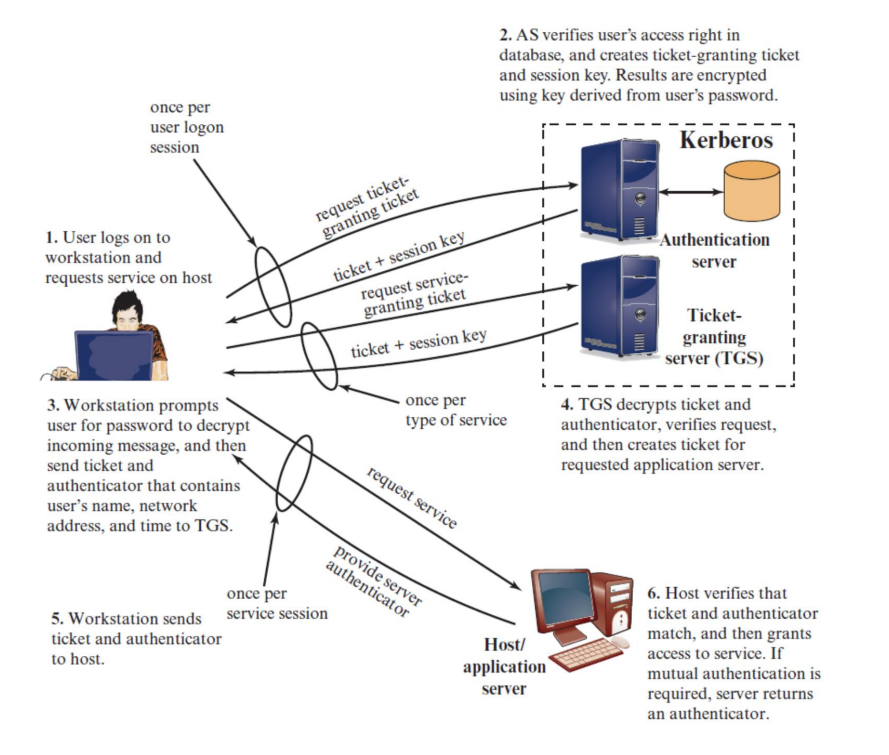
\includegraphics[width=1\textwidth]{images/chapter4/4-1.png}
    \caption{Scambio dei messaggi.}
    \label{fig:4-1}
\end{figure}

\subsection{Reami di kerberos}

Un ambiente full-service di kerberos comprende Il server Kerberos, un certo numero di client e un certo numero di server delle applicazioni. Questo tipo di ambiente vuole che:
\begin{itemize}
    \item Il server Kerberos deve avere l'ID utente e l'hash delle password di tutti gli utenti partecipanti nel suo database. Tutti gli utenti sono registrati col server Kerberos;
	\item Il server Kerberos deve condividere una chiave segreta con ciascun server TGS. Tutti i server sono registrati col server Kerberos;
	\item Il server TGS di ogni reame condivide una chiave segreta con ogni altro TGS di ogni altro reame. In questo modo le coppie di TGS si autenticano tra loro permettendo ad un utente del reame A di richiedere servizi al reame B interfacciandosi col TGS di B. Presenterà quindi a B un ticket per "risorsa esterna" emesso dal TGS di A. Il TGS di B accetterà la richiesta, rilasciando un nuovo ticket, in quanto si fida del TGS di A.
	Il ticket che il TGS di A dà al client contiene la chiave segreta condivisa tra i due TGS.
\end{itemize}
	
Il numero di chiavi condivise tra i TGS è n(n-1). Supponendo che i TGS siano 3, ogni TGS condivide 2 chiavi con gli altri, quindi il numero di chiavi totali è 6. 
Il numero limitato di chiavi e la possibilità di avere reami rendono kerberos scalabile.

\subsection{Differenze tra kerberos 4 e 5}

La versione 5 risolve alcune limitazioni della 4:
\begin{enumerate}
    \item Limiti sull'ambiente:
	\begin{itemize}
	    \item Utilizzo di AES per la cifratura (al posto di DES);
		\item Dipendenza dal protocollo Internet (non solo indirizzi IP, eventuali indirizzi di rete);
		\item Ordinamento dei byte del messaggio;
		\item Durata del ticket (durata con ora di inizio e fine esplicita nei ticket);
		\item Inoltro dell'autenticazione (visto che sono autenticato per l'uso della stampante, sono autenticato anche per le risorse che la stampante usa);
		\item Autenticazione Inter-reame (un metodo che richiede meno di $O(n^2)$ chiavi);
	\end{itemize}
    \item Limiti tecnici:
    \begin{itemize}
        \item Rimozione della doppia cifratura (analisi hanno dimostrato che non è necessario, si rimuove perché pesante);
		\item Aggiunto meccanismo di integrità:
		\item Le chiavi di sotto-sessione possono essere negoziate solo per una connessione;
		\item Preautenticazione per prevenire attacchi alle password.
    \end{itemize}
\end{enumerate}

\underline{Autenticazione mutuale}: si usa la cifratura a chiave pubblica per la distribuzione delle chiavi di sessione. La distribuzione avviene col protocollo di Dennign esteso con timestamp.

Autenticazione one-way: 
\begin{itemize}
    \item Riguarda un unico trasferimento di informazioni da un utente A ad un utente B;
	\item Stabilisce un flusso da A a B con un qualcosa che autentica il mittente;
	\item Per garantire la riservatezza il Messaggio è cifrato con una chiave one-time;
	\item La chiave one-time viene cifrata con la chiave pubblica di B, quindi solo B è in grado di recuperare la chiave e decifrare il messaggio;
	\item Questo schema (chiave one-time cifrata con chiave pubblica di B, messaggio cifrato con chiave one-time) è più efficiente che cifrare l'intero messaggio con la chiave pubblica di B;
\end{itemize}

Se mi preoccupa l'autenticazione, posso usare la firma digitale. Questo metodo garantisce che A non possa negare in seguito di aver inviato il messaggio (ma potrebbe essere che A non sia il vero originatore del massaggio). Quindi:
\begin{itemize}
    \item Oltre la messaggio, A invia a B la firma cifrata con la chiave privata di A e il certificato di A cifrato con la chiave privata dell'AS;
	\item B usa il certificato di A per ottenere la chiave pubblica di A e verifica che sia autentica;
	\item B usa quindi la chiave per verificare il messaggio;
\end{itemize}

Se è richiesta anche la confidenzialità, l'intero massaggio viene cifrato con la chiave pubblica di B oppure con una chiave one-time che viene cifrata con la chiave pubblica di B.

\section{Identità federata}
Identità comune in più aziende e numerose applicazioni. Fornisce diversi servizi come:
\begin{itemize}
    \item Punto di contatto;
	\item Servizi del protocollo SSO;
	\item Servizi fiduciari;
	\item Servizi di chiavi;
	\item Servizi di identità;
	\item Autorizzazioni;
	\item Gestione.
\end{itemize}

La gestione dell'identità consiste in un approccio centralizzato e automatizzato per fornire l'accesso alle risorse a livello aziendale da parte dei dipendenti e di altre persone autorizzate. L'obiettivo della gestione dell'identità è definire un'identità per ciascun utente (umano o processo), associare attributi all'identità e applicare un mezzo attraverso il quale un utente può verificare l'identità. Il concetto centrale del sistema è l'uso del single sign-on (SSO), che consente ad un utente di accedere a tutte le risorse di rete dopo un'unica autenticazione (figura \ref{fig:4-2}).

\begin{figure}
    \centering
    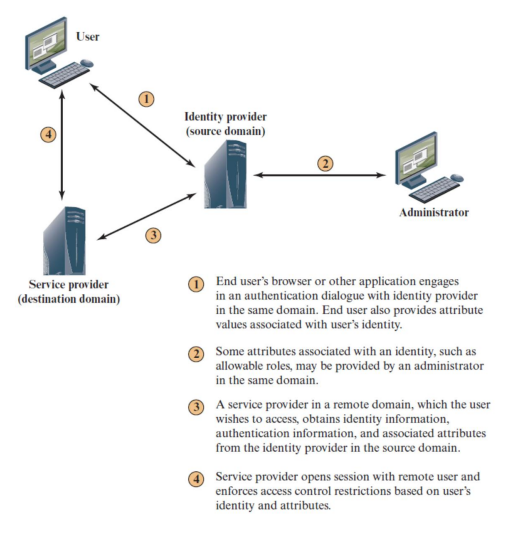
\includegraphics[width=1\textwidth]{images/chapter4/4-2.png}
    \caption{Identità federata.}
    \label{fig:4-2}
\end{figure}
\setchapterpreamble[u]{\margintoc}
\chapter{Transport Level Security}
\labch{chapter5}

Protocolli analizzati: 
\begin{itemize}
    \item TLS (standard che deriva da SSL - Socket Security Level);
	\item HTTPS e SSH, che si appoggiano a TLS.
\end{itemize}

TLS/SSL sono state create per proteggere i Web Server e rendere sicura la comunicazione col client, a causa di una serie di caratteristiche intrinseche del web:
\begin{itemize}
    \item I web server sono relativamente semplici da configurare e gestire;
	\item Il contenuto è sempre più semplice da sviluppare;
	\item L'architettura sottostante è molto complessa, e può nascondere molti buchi di sicurezza;
	\item Un web server exploitato potrebbe essere usato per attaccare la rete dell'azienda che lo possiede;
	\item Gli utenti casual e non addestrati nella sicurezza sono i clienti comuni dei servizi basati su web server.
\end{itemize}
Gli utenti devono essere protetti sa server web malevoli e viceversa.

Le minacce sul web possono violare l'integrità, la confidenzialità, la disponibilità (DDoS) e l'autenticità.

La posizione dei protocolli di sicurezza rispetto allo stack del protocollo TCP/IP è mostrata in figura \ref{fig:5-1}.

\begin{figure}
    \centering
    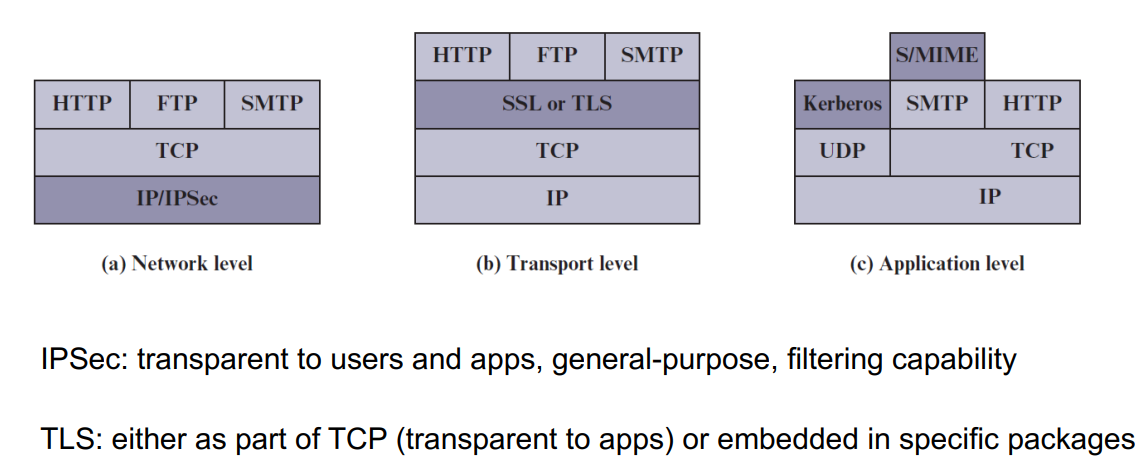
\includegraphics[width=1\textwidth]{images/chapter5/5-1.png}
    \caption{Scambio dei messaggi.}
    \label{fig:5-1}
\end{figure}

\section{Transport Level Security}
\begin{itemize}
    \item Si compone di una suite di protocolli usati in una sequenza ben precisa;
	\item È uno dei servizi di sicurezza più usati;
	\item Evolve da SSL;
	\item Si appoggia a TCP;
	\item Può venire fornito come parte del protocollo sottostante (TCP) oppure incorporato all'interno di specifici pacchetti;
	\item La maggior parte dei browser e web server lo implementano.
\end{itemize}

TLS si compone di una suit di protocolli:
\begin{itemize}
    \item Protocolli per stabilire la comunicazione e gli scambi di dati necessari ad avviare il protocollo:
	\begin{itemize}
	    \item Handshake protocol, per aprire la comunicazione tra due entità che non si conoscono  e decidere come scambiarsi le prime info necessarie alla prosecuzione del protocollo;
		\item Change chiper spec protocol, per cambiare l'algoritmo crittografico stabilito durante l'handshake;
		\item Alert protoco, per notificare situazione di warning;
		\item HTTP;
		\item Heartbeat protocol.
	\item Record protocol, che rende sicuri i dati dell'applicazione.
	\end{itemize}
\end{itemize}

L'architettura di TLS ha 2 componenti principali:
\begin{itemize}
    \item Connessione TLS: in generale una connessione è un "trasporto" che fornisce un servizio adatto al contesto in cui è stabilita. In TLS le connessioni sono relazioni peer-to-peer. Sono transienti e associate ad una sola sessione.
	\item Sessione TLS: si tratta di un'associazione tra un client e un server ed è creata tramite il protocollo di handshake. Definisce una serie di parametri crittografici per la sicurezza (lunghezza chiavi, protocollo crittografico da usare, …) condivisi tra tutte le connessioni associate alla sessione (evito di negoziare i parametri per ogni connessione).
\end{itemize}

I parametri scambiati in una sessione sono:
\begin{itemize}
    \item Identificatore della sessione;
	\item Certificato dei peer, nella versione X509.v3. Può essere nullo, in quanto il client potrebbe esserne sprovvisto;
	\item Algoritmo di compressione dei dati;
	\item Specifiche per la cifratura, come l'algoritmo di crittografia, l'algoritmo di hash per il calcolo del MAC, e altri attributi necessari alla crittografia;
	\item Master Secret, un segreto di 48 byte condiviso tra client e server;
	\item Una flag per specificare se la sessione può essere usata per aprire una nuova connessione.
\end{itemize}

I parametri di una connessione sono:
\begin{itemize}
    \item Server e client random, ovvero delle sequenze di byte scelte da client e server per ogni connessione;
	\item Server Write MAC Secret, ovvero al chiave segreta usata dal server nelle operazioni MAC sui dati inviati dal server;
	\item Client Write MAC Secret, ovvero al chiave segreta usata dal client nelle operazioni MAC sui dati inviati dal client;
	\item Server Write Key, ovvero la chiave segreta per la cifratura dei dati inviati dal server e decifrati dal client;
	\item Client Write Key, ovvero la chiave segreta per la cifratura dei dati inviati dal client e decifrati dal server;
	\item Initialization vector -> i pacchetti spediti con TLS seguono un meccanismo di block chain (la codifica di un pacchetto si basa sulla codifica del pacchetto precedente). Questo meccanismo necessita di un punto di partenza, per evitare che il primo pacchetto venga passato in chiaro, ovvero dell'initialization vector;
	\item Sequence numbers -> client e server usano delle sequenza di numeri, separate per pacchetti inviati e ricevuti, per evitare il riordino dei pacchetti da parte di un attaccante.
\end{itemize}

Obiettivi del Record Protocol:
\begin{itemize}
    \item Confidenzialità del messaggio;
	\item Integrità del messaggio.
\end{itemize}

Operazioni eseguite dal record protocol sul pacchetto:
\begin{itemize}
    \item Suddivide il pacchetto in frammenti;
	\item Comprime, senza perdere info, ciascun frammento;
	\item Calcola, per ciascun frammento compresso, il MAC e lo accoda -> integrità;
	\item Codifica il nuovo frammento -> confidenzialità;
	\item Antepone al frammento un header TLS.
\end{itemize}

\subsection{Passi dell'handshake protocol}

Nel corso di un handshake TLS, il client e il server operano insieme come segue:
\begin{itemize}
    \item Specificano la versione di TLS (TLS 1.0, 1.2, 1.3, ecc.) che utilizzeranno;
	\item Decidono quali suite di crittografia (vedi sotto) utilizzeranno;
	\item Autenticano l'identità del server tramite la chiave pubblica del server e la firma digitale dell'autorità di certificazione SSL;
	\item Generano chiavi di sessione per utilizzare la crittografia simmetrica dopo il completamento dell'handshake.
\end{itemize}

I passaggi all'interno di un handshake TLS sono (con  Diffie-Hellman autenticato):
\begin{enumerate}
    \item \textbf{'Client\_hello' e 'sever\_hello}: il client inizia l'handshake inviando un messaggio "hello" al server. Il messaggio includerà la versione TLS supportata dal client, le suite di crittografia supportate, una stringa di byte casuali che funziona come nonce e un id di sessione.
	In risposta al messaggio di saluto del client, il server invia un messaggio contenente il certificato SSL del server, la suite di cifratura scelta dal server e un suo nonce. Tipicamente è il server adatta le sue versioni di TLS e cypher suite a quelle del client o in generale ci si adatta a quello che richiede le versioni minori (Attenzione: un server/client che richiede versioni vecchie del protocollo potrebbe essere rischioso/malevolo);
	\item \textbf{Certificato e pre\_master\_secret del server}: il server invia il proprio certificato e il sua pre\_master\_secret che ha generato. Richiede, opzionalmente, al client il suo certificato;
	\item \textbf{Autenticazione e scambio chiavi}: il client verifica il certificato del server con l'autorità di certificazione che lo ha emesso. Ciò conferma che il server è chi dice di essere e che il client sta interagendo con l'effettivo proprietario del dominio. Se richiesto e se in possesso, il client può inviare il proprio certificato al server. Il client invia il proprio pre\_master\_secret;
	I due pre\_masetr\_secret vengono usati per generare il master\_secret, che sta alla base di tutte le chiavi usate durante la sessione;
	\item \textbf{Termine dell'handshake}: client e server raccolgono l'insieme di messaggi che si sono scambianti fin'ora, ne fanno l'hash (cifrato con una chiave generata a partire dal master\_secret) e verificano che i due valori ottenuti corrispondano. Questo permette di verificare che nessun attore si sia messo in mezzo allo scambio.
\end{enumerate}

 \begin{figure}
    \centering
    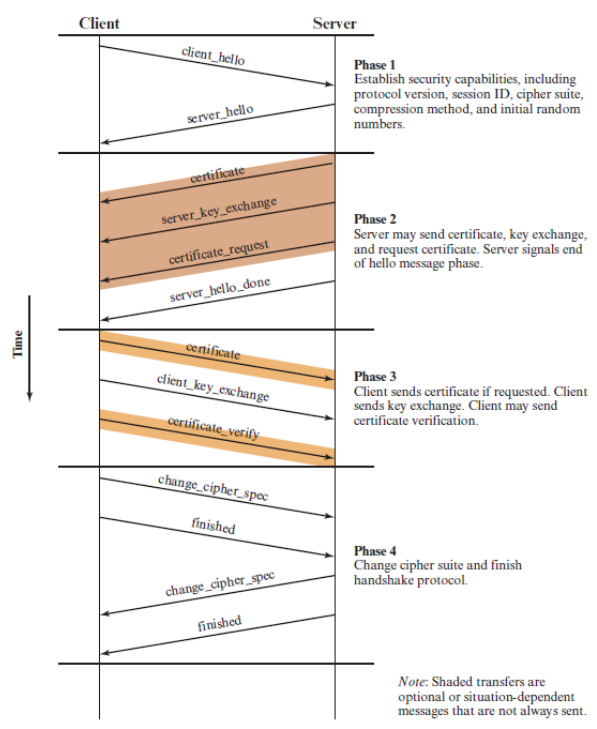
\includegraphics[width=1\textwidth]{images/chapter5/5-2.png}
    \caption{Passi dell'hasdshake protocol.}
    \label{fig:5-2}
\end{figure}

Fino all'ultima versione di SSL, il pre\_master\_secret era generato solo dal client e la crittografia usata per cifrare era RSA: 
\begin{itemize}
    \item Il server fornisce il suo certificato al client;
	\item Il client preleva la chiave pubblica del server dal certificato (dopo averlo verificato) e la usa per cifrare il pre\_master\_secret da lui generato; 
	\item Il server decifra il pre\_master\_secret ricevuto dal client  con la propria chiave privata;
	\item Entrambi i principals posseggono ora il pre\_master\_secret e possono generare il resto delle chiavi.
\end{itemize}
	
In TLS 1.3 l'suo di RSA (chiamato RSA statico) è stato deprecato, in quanto soffre di una debolezza importate: non rispetta la perfect forward secrecy. Supponiamo di aver stabilito una sessione con successo e di aver terminato l'handshake il 1° Luglio. Inizio quindi a creare delle connessioni, ognuna con la propria chiave generata a partire dalla master\_key, che durano per diverso tempo.  Il 30 di Luglio la chiave privata del server viene compromessa. Lo stesso giorno la craccatura viene scoperto e il certificato revocato. Da ora in poi infatti tutte le comunicazioni potrebbero essere compromesse. Anche le comunicazioni passate (1 - 30 Luglio) sono compromesse, in quanto l'attaccante, se ha registrato i messaggi scambiati durante l'handshake protocol, può decifrare quello contenente il pre\_master\_secret, creare il master\_secret (il metodo su come crearlo è deciso durante l'handshake) e in cascata tutte le altre chiavi. Può ora decodificare, sempre supponendo che li abbia registrati, tutti i messaggi scambiati nella sessione.

In TLS 1.3 si usa Diffie-Hellman autenticato. L'autenticazione può essere raggiunta, ad esempio, se client e server possiedono entrambi un certificato. IN questo caso ciascuno può cifrare la mezza chiave con la chiave pubblica dell'altro. A seconda del tipo di servizi/info forniti dal server, ci si può accontentare anche solo del certificato di quest'ultimo.

Nelle versioni precedente alla 1.3 di TLS,  Diffie-Hellman è comunque usabile (previo accordo tra le parti), ma non obbligatorio.

Dal master\_secret viene derivata:
\begin{itemize}
    \item Server Write MAC key;
	\item Client Write MAC key;
	\item Server Write Key;
	\item Client Write Key;
	\item Initialization vector di client e server.
\end{itemize}

Gli attacchi a TLS possono essere raggruppati in:
\begin{itemize}
    \item Attacchi all'handshake protocol;
	\item Attacchi al record protocol o ai protocolli usati dai dati dell'applicazione;
	\item Attacchi alla public key infrastructure;
    \item Altri tipi di attacchi.
\end{itemize}

\section{Secure Shell (SSH)}

Protocollo per comunicazioni di rete sicure progettato per essere relativamente semplice e poco costoso da implementare. La versione iniziale, SSH1, era focalizzata sul fornire un login da remoto sicuro su altre macchine per sostituire TELNET e altri schemi di accesso remoto che non fornivano sicurezza. 
Fornisce ora anche una capacità client/server più generale e può essere utilizzato per funzioni di rete come il trasferimento di file e la posta elettronica.
SSH2 corregge una serie di falle di sicurezza nello schema originale.

Le applicazioni client e server SSH sono ampiamente disponibili per la maggior parte dei sistemi operativi come mezzo per:
\begin{itemize}
    \item Accesso da remoto;
	\item X tunneling.
\end{itemize}

\subsection{Stack del protocollo}
Il protocollo si compone di due layer (figura \ref{fig:5-3}):
\begin{itemize}
    \item Transport Layer Protocol: fornisce l'autenticazione del server, la riservatezza dei dati, e l'integrità dei dati con forward secrecy (ad esempio, se una chiave viene compromessa durante una sessione, la sua conoscenza non minaccia la sicurezza delle sessioni precedenti). Lo strato di trasporto può opzionalmente fornire compressione;
	\item User Authentication Protocol: autentica gli utenti al server;
    \item Connection protocol.
\end{itemize}

\begin{figure}
    \centering
    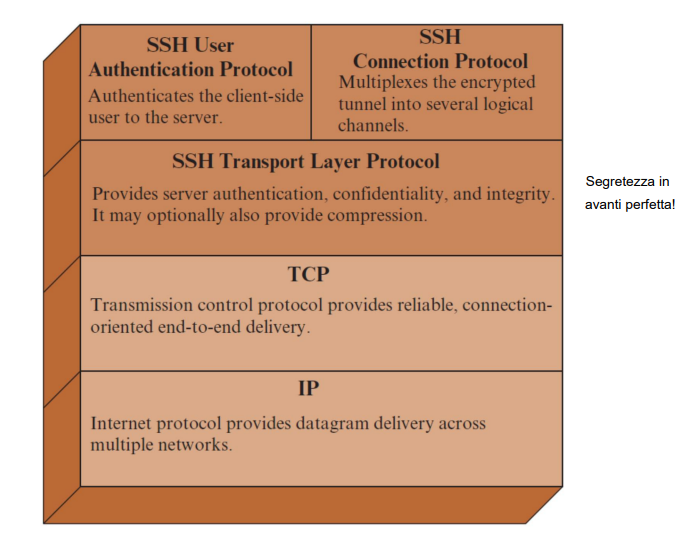
\includegraphics[width=1\textwidth]{images/chapter5/5-3.png}
    \caption{Layer SSH.}
    \label{fig:5-3}
\end{figure}

\subsection{SSH Transport Layer Protocol}

Basi:
\begin{itemize}
    \item L'autenticazione del server avviene a livello di trasporto, basandosi sul possesso di una coppia di chiavi pubblica/privata da parte del server;
	\item Un server può avere più chiavi host che utilizzano diversi algoritmi di cifratura asimmetrica;
	\item Più host possono condividere la stessa chiave host;
	\item La chiave host del server viene utilizzata durante lo scambio di chiavi per autenticare l'identità dell'host;
	\item RFC 4251 impone due modelli di trust alternativi:
	\begin{itemize}
	    \item Il client dispone di un database locale che associa ogni nome host con la chiave host pubblica corrispondente;
		\item L'associazione host-key è certificata da una Certification Authority di fiducia. Il client conosce solo la chiave radice della CA e può verificare la validità di tutte le chiavi host certificate da essa.
	\end{itemize}
\end{itemize}

\begin{figure}
    \centering
    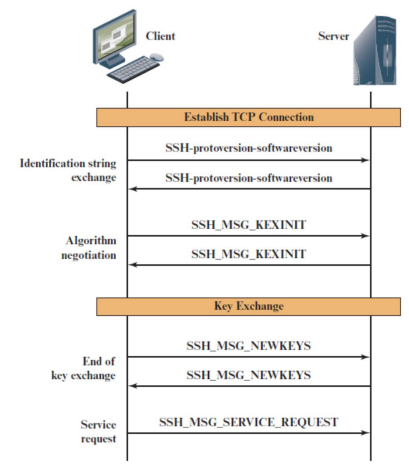
\includegraphics[width=0.9\textwidth]{images/chapter5/5-4.png}
    \caption{Scambio di messaggi in SSH Transport Layer Protocol.}
    \label{fig:5-4}
\end{figure}

Messaggi scambiati (figura \ref{fig:5-4}):
\begin{enumerate}
    \item Il client stabilisce una connessione TCP col server. Questo passo viene fatto con TCP e non con il Transport Layer Protocol;
	\item Identification string exchange: il client invia una stringa di identificazione. Il server risponde con una proprie stringa di identificazione;
	\item Algorithm negotiation: ogni parte invia una lista degli algoritmi supportati (per scambio chiavi, cifratura, MAC, compressione). Per ogni categoria, l'algoritmo scelto è il primo nella lista del client che il server supporta (il client ordina le entry della lista come vuole);
	\item Key exchange: lo scambio può avvenire con 2 versioni di Diffie-Hellman (DH). Lo scambio avviene come segue:
	\begin{enumerate}
	    \item Il client invia la sua mezza chiave di DH;
		\item Il server firma l'hash della mezza chiave, della chiave Ks e delle stringhe di identificazione con la chiave privata dell'host e invia al client la chiave pubblica dell'host Ks, l'altra mezza chiave di DH e l'hash firmato;
		\item Il client verifica la chiave pubblica dell'host KS con il suo database locale o con la CA.
	\end{enumerate}
	\item End of key exchange: si segnala la fine dello scambio con uno specifico pacchetto;
	\item Service request: il client invia un pacchetto nel quale richiede SSH User Authentication protocol o SSH Connection protocol.
\end{enumerate}

I pacchetti SSH scambiati hanno i seguenti campi:
\begin{enumerate}
    \item Lunghezza del pacchetto, escluso i campi MAC e lunghezza paccheto;
	\item Lunghezza del padding;
	\item Payload eventualmente compresso;
	\item Padding, la cui dimensione è decisa il base all'algoritmo di cifratura usato;
	\item MAC, calcolato tentendo conto di tutti i 4 campi precedenti non cifrati.
\end{enumerate}

I campi 1, 2, 3, 4 vengono cifrati con l'algoritmo scelto.

Le chiavi utilizzate per la crittografia e il MAC sono generate usando:
\begin{itemize}
    \item La chiave DH segreta condivisa K;
	\item Il valore hash usato nello scambio delle chiavi H=hash(..K..);
    \item L'identificatore di sessione, che è uguale a H a meno che non vi sia stato un successivo scambio di chiavi dopo lo scambio di chiavi iniziale.
\end{itemize}

\subsection{SSH User authentication protocol}

Il protocollo di autenticazione utente fornisce i mezzi con cui il client viene autenticato sul server. Il protocollo usa sempre tre formati di messaggi:
\begin{itemize}
    \item Messaggio del client:
	\begin{itemize}
	    \item SSH\_MSG\_USERAUTH\_REQUEST
		\item Nome utente = identità che il client dichiara
		\item Service name = struttura a cui il client sta richiedendo l'accesso (generalmente SSH Connection Protocol)
		\item Method name = metodo di autenticazione utilizzato nella richiesta
	\end{itemize}
	\item Risposta negativa del server:
	\begin{itemize}
	    \item SSH\_MSG\_USERAUTH\_FAILURE
		\item Lista di metodi che potrebbero continuare il dialogo
		\item Booleano che indica il parziale successo
	\end{itemize}
	\item Risposta positiva del server:
	\begin{itemize}
	    \item SSH\_MSG\_ USERAUTH\_SUCCESS
	\end{itemize}
\end{itemize}

\begin{figure}
    \centering
    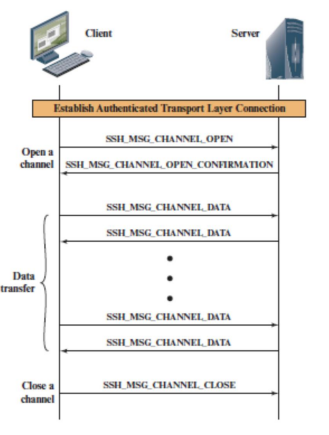
\includegraphics[width=0.9\textwidth]{images/chapter5/5-5.png}
    \caption{Scambio di messaggi per SSH User authentication protocol.}
    \label{fig:5-5}
\end{figure}

Scambio dei messaggi (figura \ref{fig:5-5}):
\begin{enumerate}
    \item Il cliente invia a SSH\_MSG\_USERAUTH\_REQUEST senza specificare il method name;
	\item Il server verifica se il nome utente è valido. In caso contrario, il server restituisce SSH\_MSG\_USERAUTH\_FAILURE con il valore di successo parziale false. Se il nome utente è valido, il server procede al passaggio 3;
	\item Il server restituisce SSH\_MSG\_USERAUTH\_FAILURE con un elenco di uno o più metodi di autenticazione da utilizzare;
	\item Il client seleziona uno dei metodi di autenticazione e invia un SSH\_MSG\_USERAUTH\_REQUEST con il nome del metodo e i campi specifici del metodo richiesti. A questo punto, potrebbe esserci una sequenza di scambi per eseguire il metodo;
	\item Se l'autenticazione ha esito positivo e sono necessari più metodi di autenticazione, il server procede al passaggio 3, utilizzando il valore di successo parziale true. Se l'autenticazione non riesce, il server procede al passaggio 3, utilizzando il valore di successo parziale false;
	\item Quando tutti i metodi di autenticazione richiesti hanno esito positivo, il server invia un messaggio SSH\_MSG\_USERAUTH\_SUCCESS e il protocollo di autenticazione è terminato.
\end{enumerate}

Metodi di autenticazione:
\begin{itemize}
    \item Chiave pubblica: 
	\begin{itemize}
	    \item Il client invia un messaggio al server che contiene la chiave pubblica del client, con il messaggio firmato con la chiave privata del client;
		\item Quando il server riceve il messaggio, verifica se la chiave fornita è accettabile per l'autenticazione e, in caso affermativo, verifica se la firma è corretta.
	\end{itemize}
	\item Password: 
	\begin{itemize}
	    \item Il client invia un messaggio contenente una password in chiaro, cifrata dal Transport Layer Protocol (TLS);
	\end{itemize}
	\item Attraverso l'hosh:
	\begin{itemize}
	    \item L'autenticazione viene eseguita sull'host del client anziché sul client stesso;
		\item Questo metodo funziona facendo in modo che il client invii una firma creata con la chiave privata dell'host;
		\item Anziché verificare direttamente l'identità dell'utente, il server SSH verifica l'identità dell'host (perdo l'accountability in quanto non so chi è effettivamente connesso all'host).
	\end{itemize}
\end{itemize}

\subsection{SSH Connection Protocol}

Il protocollo di connessione SSH viene eseguito sopra l'SSH Transport Layer Protocol e presuppone che sia attiva una connessione autenticata sicura. La connessione di autenticazione sicura, denominata tunnel, viene utilizzata dal protocollo di connessione per multiplexare un numero di canali logici.

Canale:
\begin{itemize}
    \item Tutti i tipi di comunicazione tramite SSH sono supportati utilizzando canali separati;
	\item Entrambe le parti possono aprire un canale;
	\item Ad ogni canale, ogni lato associa un numero di canale univoco;
	\item Il flusso dei canali è controllato mediante un meccanismo a finestra;
	\item Nessun dato può essere inviato a un canale finché non viene ricevuto un messaggio che indica che lo spazio della finestra è disponibile;
	\item La vita di un canale procede attraverso tre fasi: apertura del canale, trasferimento dati, chiusura del canale.
\end{itemize}

Messaggi scambiati:
\begin{enumerate}
    \item \textbf{Apertura del nuovo canale}: la parte che desidera aprire il canale allora un numero locale per il canale e invia un messaggio di apertura, che contiene:
	\begin{itemize}
	    \item SSH\_MSG\_CHANNEL\_OPEN
		\item Tipo del canale, che identifica l'applicazione per il canale
		\item Il numero locale del canale
		\item Dimensione iniziale della finestra
		\item Dimensione massima dei pacchetti
		\item Info sui dati
	\end{itemize}
	2. Se l'altra parte è in grado di aprire il canale, invia un messaggio di conferma che contiene:
	\begin{itemize}
	    \item SSH\_MSG\_CHANNEL\_OPEN\_CONFIRMATION
		\item Il numero locale ricevuto
		\item Il numero locale allocato
		\item Dimensione della finestra e dei pacchetti per il traffico in entrata
	\end{itemize}
	In caso di insuccesso nell'apertura, il messaggio contiene:
	\begin{itemize}
	    \item SSH\_MSG\_CHANNEL\_OPEN\_FAILURE
		\item Codice che rappresenta il motivo del fallimento
	\end{itemize}
	\item \textbf{Data transfer}: scambio di dati tra le due parti;
	\item \textbf{Chiusura canale}: la parte che desidera chiudere il canale invia un messaggio a riguardo.
\end{enumerate}

Tipi di canale:
\begin{itemize}
    \item Sessione: esecuzione remota di un programma. Il programma può essere una shell, un'applicazione come il trasferimento di file o e-mail, un comando di sistema o un sottosistema integrato. Una volta aperto un canale di sessione, le richieste successive vengono utilizzate per avviare il programma remoto;
	\item X11: Si riferisce a X Window System, un sistema software per computer e un protocollo di rete che fornisce un'interfaccia utente grafica (GUI) per i computer in rete. X consente alle applicazioni di essere eseguite su un server di rete ma di essere visualizzate su una macchina desktop;
	\item Forwarded-tcpip: forwarding remoto della porta;
	\item Direct-tcpip: forwarding della porta locale.
\end{itemize}

Port forwarding (inoltro della porta):
\begin{itemize}
    \item Una delle funzionalità più utili di SSH;
	\item Offre la possibilità di convertire qualsiasi connessione TCP non sicura in una connessione SSH sicura (denominato anche tunneling SSH);
	\item Il traffico TCP in entrata viene consegnato all'appropriata applicazione in base al numero di porta (una porta è un identificatore di un utente di TCP);
	\item Un'applicazione può utilizzare più numeri di porta.
\end{itemize}

Supponiamo di avere un'applicazione client identificata dal numero di porta x e un'applicazione server identificata dal numero di porta y. Ad un certo punto, l'applicazione client richiama l'entità TCP locale e richiede una connessione al server remoto sulla porta y. L'entità TCP locale negozia una connessione TCP con l'entità TCP remota, in modo tale che la connessione colleghi la porta locale x alla porta remota y.

Per proteggere questa connessione, SSH è configurato in modo che SSH Transport Layer Protocol stabilisca una connessione TCP tra le entità client e server SSH, rispettivamente con i numeri di porta TCP a e b. Un tunnel SSH sicuro viene stabilito su questa connessione TCP. Il traffico dal client alla porta x viene reindirizzato all'entità SSH locale e viaggia attraverso il tunnel in cui l'entità SSH remota consegna i dati all'applicazione server sulla porta y. Il traffico nella direzione opposta viene reindirizzato in modo simile.

\begin{figure}
    \centering
    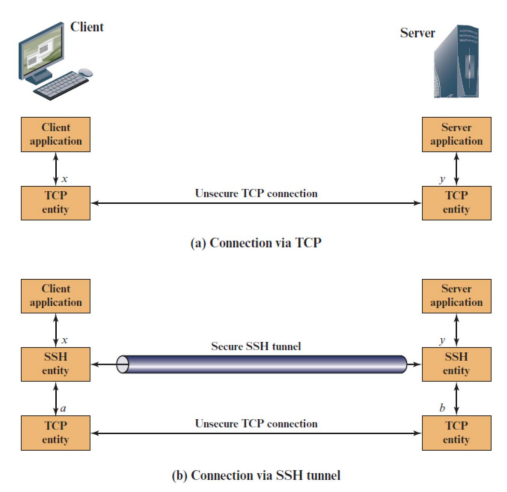
\includegraphics[width=1\textwidth]{images/chapter5/5-6.png}
    \caption{Scambio di messaggi per SSH User authentication protocol.}
    \label{fig:5-6}
\end{figure}

\section{Appunti aggiuntivi}

\subsection{Rollback attack in SSL}

La versione originale di SSL 3.0 prevedeva, nella fase iniziale dell'handshake, l'invio in chiaro da parte del client della versione di SSL supportata, insieme alle altre info di configurazione. Se il messaggio veniva catturato prima di arrivare al server, l'attaccante poteva facilmente modificare impostazioni come la versione, essendo non cifrata, inserendo ad esempio la versione 2.0, che non supporta il controllo con hash finale dello scambio di messaggi.
Per risolvere, SSL 3.0 ha deciso che il client, nel successivo messaggio che contiene la mezza chiave, vada ad inserire anche la versione di SSL che lui sta utilizzando. Ovviamente questo messaggio è cifrato con la chiave pubblica del server, e quindi sicuro.

\subsection{Combinare HTTPS con HTTP}

Tralasciando i casi di errori di programmazione dove uno script attiva erroneamente HTTP, esistono casi in cui i siti web accettano di servire sia HTTP che HTTPS (es: arrivo al sito con HTTP, vengo rediretto al login con HTTPS; cerco nel sito con HTTP, vado al checkout con HTTPS). In questi casi l'attaccante, se riesce a catturare il messaggio del client, può modificarne il contenuto sostituendo la richiesta del protocollo HTTPS con quello HTTP.

\subsection{Vulnerabilità nel salvataggio delle chiavi}

La chiave privata può essere protetta nel server in più modi:
\begin{itemize}
    \item  Usando uno specifico HW che genera coppie di chiavi SSL, mantiene la chiave privata e si occupa della cifratura. L'HW è costoso e richiede specifici driver nel server;
	\item Mantenendo la chiave sul server cifrata;
	\item Mantenendo la chiave sul server non cifrata (MOLTO comune).
\end{itemize}
 
\subsection{Vulnerabilità nella gestione dei certificati}

Se un nodo della catena è compromesso, tutto il sottoalbero è compromesso.



\setchapterpreamble[u]{\margintoc}
\chapter{Wireless Network Security}
\labch{chapter6}

Fattori che rendono più rischiose le reti wireless rispetto a quelle cablate:
\begin{itemize}
    \item Canale: 
	\begin{itemize}
	    \item Le reti wireless in genere implicano comunicazioni broadcast, che sono molto più soggette a intercettazioni e disturbi rispetto alle reti cablate;
		\item Le reti wireless sono anche più vulnerabili agli attacchi attivi che sfruttano le vulnerabilità nei protocolli di comunicazione (Jamming);
	\end{itemize}
	\item Mobilità:
	\begin{itemize}
	    \item I dispositivi wireless sono molto più portatili e mobili rispetto ai dispositivi collegati con cavo. La mobilità comporta una serie di rischi;
	\end{itemize}
	\item Risorse:
	\begin{itemize}
	    \item Alcuni dispositivi wireless, come smartphone e tablet, dispongono di sistemi operativi sofisticati ma memoria e risorse di elaborazione limitate con cui contrastare le minacce, inclusi DDoS e malware;
	\end{itemize}
	\item Accessibilità:
	\begin{itemize}
	    \item Alcuni dispositivi wireless, come sensori e robot, potrebbero essere lasciati incustoditi in luoghi remoti e/o ostili, rendendoli più deboli ad attacchi fisici.
	\end{itemize}
\end{itemize}

\begin{figure}[h]
    \centering
    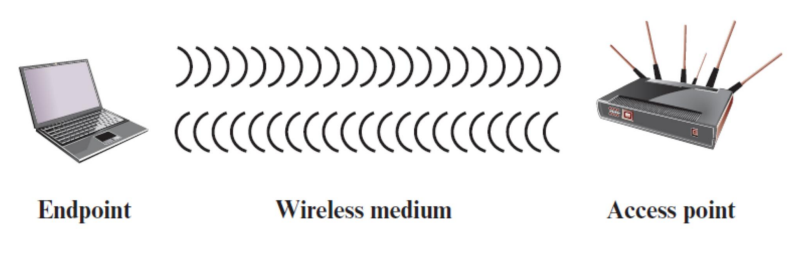
\includegraphics[width=1\textwidth]{images/chapter6/6-1.png}
    \caption{Reti wireless.}
    \label{fig:6-1}
\end{figure}

Minacce alle reti wireless:
\begin{itemize}
    \item Associazione accidentale: 
	\begin{itemize}
	    \item Wireless LAN aziendali create vicine tra loro potrebbero creare dei campi di trasmissione sovrapposti;
		\item Un utente che intende connettersi a una LAN potrebbe bloccarsi involontariamente su un punto di accesso wireless da una rete vicina;
	\end{itemize}
	\item Associazione dannosa: un dispositivo wireless è configurato per apparire come un access point legittimo, consentendo all'operatore di rubare le password di utenti legittimi e quindi penetrare in una rete cablata attraverso un punto di accesso wireless legittimo;
	\item Reti ad-hoc: si tratta di reti peer-to-peer tra computer wireless senza punti di accesso tra di loro. Possono rappresentare una minaccia per la sicurezza a causa della mancanza di un punto centrale di controllo;
	\item Reti non tradizionali: reti e collegamenti non tradizionali, come dispositivi Bluetooth di rete personale, lettori di codici a barre e palmari, rappresentano un rischio per la sicurezza sia in termini di intercettazione che di spoofing;
	\item MAC spoofing (furto di identità): si verifica quando un utente malintenzionato è in grado di intercettare il traffico di rete e identificare l'indirizzo MAC di un computer con privilegi di rete;
	\item Attacchi man-in-the-middle: questo attacco consiste nel persuadere un utente e un punto di accesso a credere che stiano parlando tra loro quando in realtà la comunicazione sta attraversando un dispositivo di attacco intermedio. Le reti wireless sono particolarmente deboli a questi attacchi;
	\item DDoS: questo attacco si verifica quando un utente malintenzionato bombarda continuamente un punto di accesso wireless o qualche altra porta wireless accessibile con vari messaggi di protocollo progettati per consumare risorse di sistema. L'ambiente wireless si presta a questo tipo di attacco perché è facile per l'attaccante indirizzare più messaggi wireless verso il bersaglio;
	\item Network injection: prende di mira i punti di accesso wireless che sono esposti a traffico di rete non filtrato, come messaggi del protocollo di instradamento o messaggi di gestione della rete.
\end{itemize}
		
Protezione delle trasmissioni wireless:
\begin{itemize}
    \item Le principali minacce alla trasmissione wireless sono le intercettazioni, le alterazione o inserimento di messaggi e interruzioni;
	\item Per affrontare le intercettazioni, esistono due tipi di contromisure:
	\begin{enumerate}
	    \item Tecniche di occultamento del segnale:
		\begin{itemize}
		    \item Disattivare la trasmissione SSID dai punti di accesso wireless;
			\item Assegnare nomi criptici agli SSID;
			\item Ridurre la potenza del segnale al livello più basso che fornisce comunque la copertura richiesta;
			\item Piazzare i punti di accesso wireless all'interno dell'edificio, lontano da finestre e pareti esterne.
		\end{itemize}
		\item Cifratura:
		\begin{itemize}
		    \item È efficace contro le intercettazioni nella misura in cui le chiavi sono protette.
		\end{itemize}
	\end{enumerate}
\end{itemize}

Protezione dei punti di accesso:
\begin{itemize}
    \item La principale minaccia che coinvolge i punti di accesso wireless è l'accesso non autorizzato alla rete;
	\item L'approccio principale per impedire tale accesso è lo standard IEEE 802.1x per il controllo dell'accesso alla rete basato su porte. L'uso di 802.1X può impedire che punti di accesso non autorizzati e altri dispositivi non autorizzati diventino backdoor non sicuri.
\end{itemize}

Raccomandazioni per la protezione delle reti wireless:
\begin{itemize}
    \item Usare la crittografia;
	\item Utilizzare software antivirus, antispyware e firewall;
	\item Disattivare la trasmissione broadcast dell'identificatore;
	\item Modificare l'identificatore sul router rispetto a quello predefinito;
	\item Modificare la password preimpostata del router;
	\item Consenti solo a computer specifici di accedere alla rete wireless.
\end{itemize}

\section{Sicurezza dei dispositivi mobili}

I dispositivi mobili sono diventati un elemento essenziale per le organizzazioni come parte dell'infrastruttura di rete complessiva. Prima dell'uso diffuso degli smartphone, la sicurezza della rete si basava su perimetri chiaramente definiti che separavano le reti interne affidabili da Internet. A causa di enormi cambiamenti, le reti di un'organizzazione devono ora ospitare: un uso crescente di dispositivi, applicazioni cloud, deperimetrizzazione, requisiti aziendali esterni (ospiti in visita).

Problemi principali per la sicurezza dei dispositivi mobili:
\begin{itemize}
    \item Utilizzo di app create da sconosciuti: è facile trovare e installare applicazioni di terze parti sui dispositivi mobili e ciò comporta il rischio di installare software dannoso;
	\item Interazione con altri sistemi: a meno che un'organizzazione non abbia il controllo di tutti i dispositivi coinvolti nella sincronizzazione, esiste un rischio considerevole che i dati dell'organizzazione vengano archiviati in una posizione non protetta, oltre al rischio di introduzione di malware;
	\item Utilizzo dei servizi di localizzazione: un utente malintenzionato può utilizzare le informazioni sulla posizione per determinare dove si trovano il dispositivo e l'utente.
\end{itemize}

\paragraph{Policy bring-your-own-device} Se l'utente può portare a casa il dispositivo aziendale, è necessario che l'azienda implementi una forte policy di sicurezza, per evitare che il dispositivo o la rete, quando il dispositivi viene ricollegato, vengano attaccati. Implemento quindi una:
\begin{itemize}
    \item Sicurezza nel dispositivi: blocco automatico, antivirus, PIN;
	\item Sicurezza nel traffico della rete: TLS, autenticazione forte, VPN;
	\item Barriere all'ingresso della rete: firewall, IDS.
\end{itemize}

\section{Standard IEEE 802.11}

IEEE 802 è un comitato che ha sviluppato standard per un'ampia gamma di reti locali (LAN). Nel 1990 il Comitato IEEE 802 ha formato un nuovo gruppo di lavoro, IEEE 802.11, per sviluppare un protocollo e specifiche di trasmissione per LAN wireless (WLAN). 

Definizioni:
\begin{enumerate}
    \item Access Point (AP): qualsiasi entità che dispone della funzionalità della stazione e fornisce l'accesso al sistema tramite il supporto wireless per le stazioni associate;
	\item Basic Service Set (BSS): insieme di stazioni controllate da un'unica coordination function;
	\item Coordination Function: funzione logica che determina quando una stazione operante all'interno di un BSS è autorizzata a trasmettere e può essere in grado di ricevere PDU;
	\item Distribution System (DS): sistema utilizzato per interconnettere un insieme di BSS e LAN integrate per creare un ESS;
	\item Extended Service Set (ESS): insieme di uno o più BSS interconnessi e LAN integrate che appaiono come un singolo BSS al livello LLC in qualsiasi stazione associata a uno di questi BSS;
	\item MAC protocol data unit (MPDU): unità di dati scambiati tra due entità MAC peer utilizzando i servizi del livello fisico;
	\item MAC service data unit (MSDU): informazioni consegnate come unità tra utenti MAC;
	\item Stazione: Qualsiasi dispositivo che contenga un MAC e un layer fisico conforme a IEEE 802.11.
\end{enumerate}

\subsection{Stack del protocollo IEEE 802.11}

\begin{figure}[h]
    \centering
    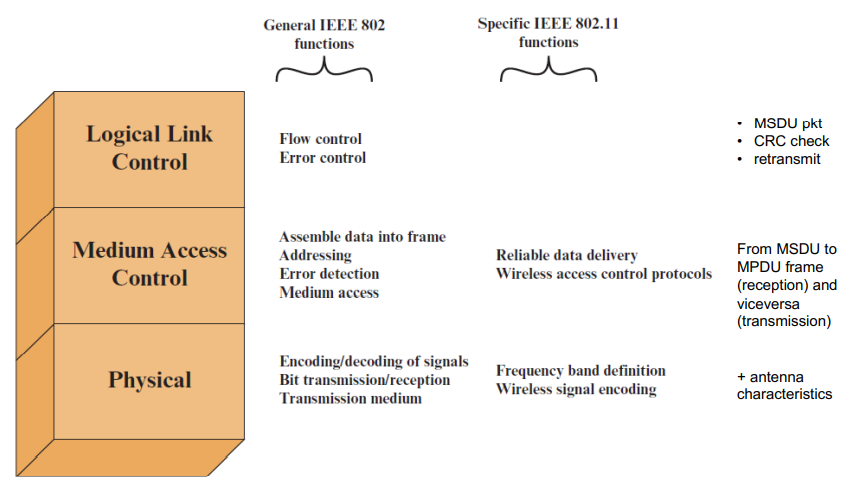
\includegraphics[width=1\textwidth]{images/chapter6/6-2.png}
    \caption{Stack del protocollo IEEE 802.11.}
    \label{fig:6-2}
\end{figure}

\begin{itemize}
    \item Logical link control:
	\begin{itemize}
	    \item 802 -> controllo del flusso, controllo degli errori;
	\end{itemize}
	\item Medium Access Control:
	\begin{itemize}
	    \item 802 -> assembra i dati in frame, indirizzamento, individuazione degli errori, accesso al medium;
		\item 802.11 -> consegna affidabile, protocolli di access control wireless;
	\end{itemize}
	\item Layer fisico:
	\begin{itemize}
	    \item 802 -> encoding/decoding del segnale, trasmissione/ricezione dei bit;
		\item 802.11 -> definizione della frequenza della banda, encoding del segnale wireless.
	\end{itemize}
\end{itemize}

\subsection{Formato MPDU in IEEE 802}

\begin{figure}[h]
    \centering
    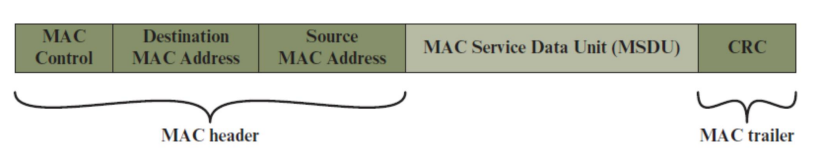
\includegraphics[width=1\textwidth]{images/chapter6/6-3.png}
    \caption{Formato MPDU in IEEE 802.}
    \label{fig:6-3}
\end{figure}

Campi:
\begin{itemize}
    \item MAC control: info di controllo del protocollo come livello di priorità;
	\item Indirizzo MAC di destinazione: indirizzo fisico di destinazione sulla LAN;
	\item Indirizzo MAC di origine: indirizzo fisico di origine sulla LAN;
	\item MSDU: dati dal livello successivo superiore;
	\item CRC (Cyclic redundancy check): ridondanza ciclica, campo di controllo sui bit dell'intera MDPU.
\end{itemize}

\subsection{IEEE 802.11 Extended Service Set (EES)} 

\begin{figure}[h]
    \centering
    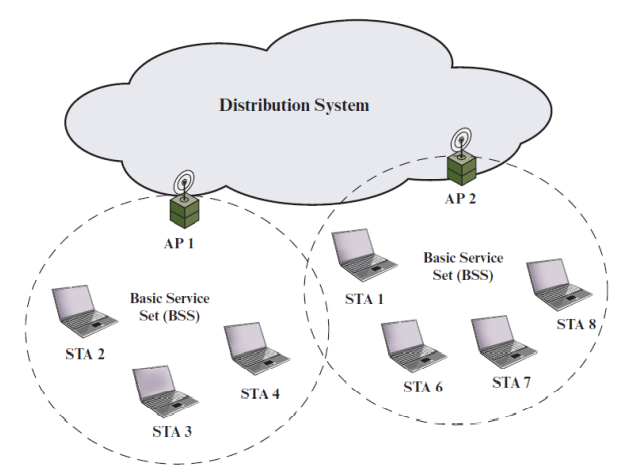
\includegraphics[width=1\textwidth]{images/chapter6/6-4.png}
    \caption{IEEE 802.11 Extended Service Set (EES).}
    \label{fig:6-4}
\end{figure}

\subsection{Servizi IEEE 802.11}

I servizi per la distribuzione dei messaggi all'interno del DS sono:
\begin{itemize}
    \item Distribution: servizio principale utilizzato dalle stazioni per lo scambio MPDU quando le MPDU devono attraversare il DS per andare da una stazione in un BSS a una stazione in un altro BSS;
	\item Integration: consente il trasferimento di dati tra una stazione su una LAN IEEE 802.11 e una stazione su una LAN IEEE 802.x integrata (cablata). Si occupa di ogni traduzione degli indirizzi e delle logiche di conversione dei media necessarie per lo scambio dei dati.
\end{itemize}

Per quanto riguarda i servizi relativi all'associazione, lo standard definisce 3 tipi di transizioni:
\begin{itemize}
    \item Nessuna transizione: la stazione è fissa o si muove solo all'interno del raggio di comunicazione diretta delle stazioni comunicanti di un singolo BSS;
	\item Transizione BSS: movimento della stazione da un BSS a un altro BSS all'interno dello stesso ESS. La consegna dei dati alla stazione richiede che la capacità di indirizzamento sia in grado di riconoscere la nuova posizione della stazione;
	\item Transizione ESS: spostamento della stazione da un BSS in un ESS a un BSS all'interno di un altro ESS. È probabile che si verifichi un'interruzione del servizio.
\end{itemize}

Per recapitare un messaggio all'interno di un DS, il servizio di distribuzione deve conoscere l'identità dell'AP a cui deve essere consegnato il messaggio affinché il messaggio raggiunga la stazione di destinazione. 
I servizi che si occupano di mantenere l'associazione della stazione all'Access Point all'interno del BSS corrente sono:
\begin{itemize}
    \item Associazione: stabilisce un'associazione iniziale tra stazione e AP;
	\item Riassociazione: permette di trasferire un'associazione già stabilita da un AP ad un altro, permettendo ad una stazione di passare da un BSS a un altro;
	\item Disassociazione: notifica da parte della stazione o dell'AP che l'associazione esistente è terminata.
\end{itemize}

\subsection{Sicurezza delle WLAN - IEEE 802.11i}

I servizi di protezione delle WLAN adottati sono:
\begin{itemize}
    \item Wired Equivalent Privacy (WEP): porzione relativa alla privacy dello standard IEEE 802.11. Conteneva gravi debolezze;
	\item Wi-Fi Protected Access (WAP): insieme di meccanismi di sicurezza che elimina la maggior parte dei problemi di sicurezza 802.11. Basato sullo stato attuale dello standard 802.11i;
	\item Robust Network Security (RNS o WAP2/WAP3): forma finale dello standard IEEE 802.11i 2012. Molto complesso. Garantisce:
	\begin{itemize}
	    \item Access Control;
		\item Autenticazione e generazione delle chiavi;
		\item Confidenzialità, autenticazione dell'origine dei dati, integrità e protezione dai replay attack.
	\end{itemize}
\end{itemize}

Fasi operative della sicurezza stazione-Access Point
\begin{enumerate}
    \item \textbf{Discovery}: l'AP invia messaggi beacon per dire che esiste. La stazione che vuole collegarsi risponde e si associa, scegliendo, tra le proposte inserite nel beacon, il cypher suite e il meccanismo di autenticazione da usare;
	\item \textbf{Authentication}: durante questa fase, la STA e l'Authentication Server si identificano reciprocamente. l'AP blocca il traffico di non autenticazione tra STA e AS finché l'autenticazione non riesce .L'unica cosa che fa AP in questa fase è inoltrare traffico tra STA e AS;
	\item \textbf{Key management}: l'AP e la STA eseguono diverse operazioni che determinano la generazione e il posizionamento di chiavi crittografiche sull'AP e sulla STA. I frame vengono scambiati solo tra AP e STA;
	\item \textbf{Protected Data Transfer}: i frame vengono scambiati tra la STA e la stazione finale tramite l'AP. Il trasferimento sicuro dei dati avviene solo tra la STA e l'AP (come indicato dall'ombreggiatura e dall'icona del modulo di crittografia); la sicurezza non è fornita end-to-end. Infatti le chiavi crittografiche se le sono scambiate la stazione e l'AP, quindi la comunicazione sarà STA -> AP, AP -> STA2;
	\item \textbf{Connection termination}: la connessione protetta viene interrotta e la connessione viene ripristinata allo stato originale.
\end{enumerate}

\begin{figure}[h]
    \centering
    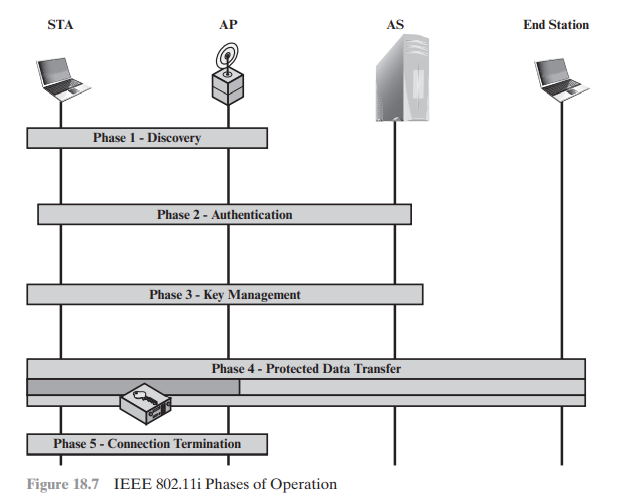
\includegraphics[width=1\textwidth]{images/chapter6/6-5.png}
    \caption{Fasi IEEE 802.11i.}
    \label{fig:6-4}
\end{figure}

Lo scopo di questa fase è che una STA e un AP si riconoscano, si accordino su una serie di capacità di sicurezza e stabiliscano un'associazione per la comunicazione futura utilizzando tali capacità di sicurezza. I passi di questa fase sono:
\begin{enumerate}
    \item \textbf{Probe request/response}: la STA risponde al beacon dell'AP, proponendosi alla connessione. L'AP trasmette periodicamente le proprie capacità di sicurezza in un canale specifico attraverso il Beacon. Le capacità di sicurezza non sono negoziabili, quindi se la STA non le accetta la connessione termina;
	\item \textbf{Open system authentication}: i due dispositivi (STA e AP) si scambiano semplicemente degli identificatori. Questo passo è necessario per garantire la compatibilità con le versioni precedenti di 802.11;
	\item \textbf{Association}: la STA invia un frame di richiesta di associazione all'AP. In questo passo, la STA specifica un insieme di funzionalità (autenticazione e gestione delle chiavi, crittografia) tra quelle pubblicizzate dall'AP. Se non c'è corrispondenza nelle capacità tra l'AP e la STA, l'AP rifiuta la richiesta di associazione;
\end{enumerate}

\begin{figure}[h]
    \centering
    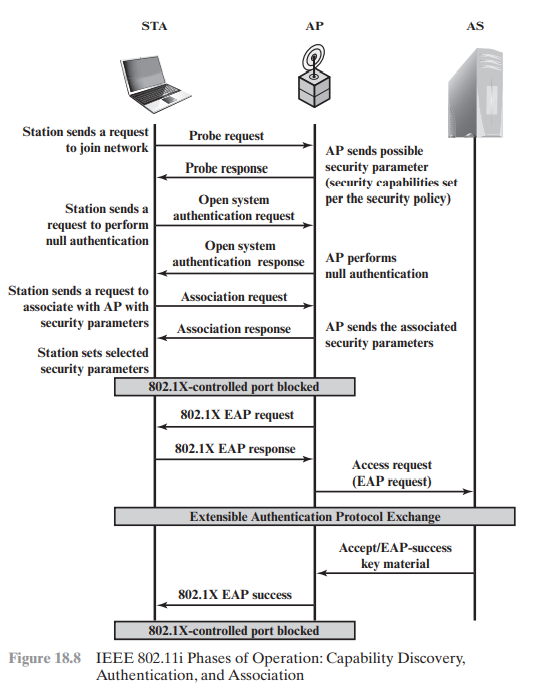
\includegraphics[width=1\textwidth]{images/chapter6/6-6.png}
    \caption{Fasi IEEE 802.11i (pt.2).}
    \label{fig:6-4}
\end{figure}

La fase di autenticazione consente l'autenticazione reciproca tra una STA e un server di autenticazione (AS) situato nel DS. L'autenticazione è progettata per consentire solo alle stazioni autorizzate di utilizzare la rete e per fornire alla STA la certezza che sta comunicando con una rete legittima. L'autenticazione viene effettuata tramite il protocollo EAP (Extensible Authentication Protocol).
L'AS si trova generalmetne len lato cablato della rete, anche se a volte può essere nell'AP.
L'AS genera una Master Session Key (MSK) e invia alla STA tramite EAP. Tutte le altre chiavi sono generate a partire dalla MSK.

A partire dalla master key, vengono generate una serie di chiavi, che possono essere divise in 2 tipologie:
\begin{itemize}
    \item Per comunicazioni simmetriche point to point da un dispositivo ad un altro (comunicazioni pairwise);
	\item Per comunicazioni di gruppo (broadcast, le chiavi sono comuni al gruppo).
\end{itemize}

Per il trasferimento protetto dei dati, IEEE 802.11i definisce due possivili schemi:
\begin{itemize}
    \item Tempora Key Integrity Protocol (TKIP): ora deprecato, è stato progettato per richiedere solo modifiche software ai dispositivi implementati con WEP. Fornisce due servizi:
	\begin{itemize}
	    \item Integrità del messaggio: aggiunge un codice di integrità del messaggio (MIC) al frame;
		\item Riservatezza dei dati: MPDU + MIC sono crittografati utilizzando RC4.
	\end{itemize}
	\item Counter Mode-CBC MAC Protocol (CCMP): destinato ai dispositivi IEEE 802.11 più recenti che sono dotati dell'hardware per supportarlo. Fornisce due servizi:
	\begin{itemize}
	    \item Integrità del messaggio: utilizza il MAC concatenamento di blocchi di crittografia;
		\item Riservatezza dei dati: utilizza la modalità di cifratura a blocchi CTR con AES.
	\end{itemize}
\end{itemize}

Per la generazione delle chiavi vengono usare pseudorandom function.

\setchapterpreamble[u]{\margintoc}
\chapter{Network security endpoint}
\labch{chapter7}


\section{Firewall}

Tipicamente inserito tra la rete e Internet o all'interno della rete per isolarne delle porzioni. 

Scopo:  creare un perimetro esterno di sicurezza che protegga la rete dagli attacchi tramite internet, fornire un unico punto dove settare sicurezza e auditing, isolare sezioni della rete dalla rete stessa o dall'esterno.

Funzionamento ad alto livello: 
\begin{itemize}
    \item Tutto il traffico dall'interno verso l'esterno, e viceversa, passa attraverso il firewall. Ciò si ottiene bloccando fisicamente tutti gli accessi alla rete locale eccetto tramite il firewall;
	\item Solo il traffico autorizzato, come definito dalla security policy locale, può passare. Diversi tipi di firewall possono usare diversi tipi di policy;
	\item Il firewall stesso deve essere immune alla penetrazione. Ciò implica l'uso di un sistema rinforzato con un sistema operativo protetto. I sistemi informatici affidabili sono adatti per ospitare un firewall e sono spesso richiesti nelle applicazioni governative.
\end{itemize}

Tecniche utilizzate dai firewall per controllare l'accesso e applicare la politica di sicurezza decisa:
\begin{itemize}
    \item Controllo sul servizio: determina i tipi di servizi Internet che possono essere accessibili, in entrata o in uscita (posso avere policy diverse per entrata e uscita);
	\item Controllo sulla direzione: determina la direzione in cui le richieste di un particolare servizio possono essere avviate e consentite a fluire attraverso il firewall;
	\item Controllo sull'utente: controlla l'accesso a un servizio in base a quale utente sta tentando di accedervi;
	\item Controllo sul comportamento: controlla come vengono utilizzati determinati servizi.
\end{itemize}

Funzionalità:
\begin{itemize}
    \item Un firewall definisce un unico punto di strozzatura che tiene gli utenti non autorizzati fuori dalla rete protetta, impedisce a servizi potenzialmente vulnerabili di entrare o uscire dalla rete e fornisce protezione da vari tipi di attacchi IP spoofing e di routing;
	\item Un firewall fornisce una posizione per il monitoraggio di eventi relativi alla sicurezza (audit, allarmi, ecc.);
	\item Un firewall è una piattaforma conveniente per diverse funzioni Internet non correlate alla sicurezza (NAT, log sull'uso di internet, …);
	\item Un firewall può fungere da piattaforma per l'implementazione di virtual private network.
\end{itemize}

Limiti del firewall:
\begin{itemize}
    \item  Il firewall non può proteggere da attacchi che aggirano il firewall;
	\item Il firewall potrebbe non proteggere completamente dalle minacce interne, come un dipendente scontento o un dipendente che collabora inconsapevolmente con un aggressore esterno;
	\item È possibile accedere a una wireless LAN protetta in modo non corretto dall'esterno dell'organizzazione. Un firewall interno che separa porzioni della rete aziendale non può proteggere dalle comunicazioni wireless tra sistemi locali su lati diversi del firewall interno;
	\item Il firewall non può proteggere da dispositivi infettati fuori dalla rete aziendale che vengono successivamente connessi e usati.
\end{itemize}

\subsection{Firewall packet filter}

\begin{figure}[h]
    \centering
    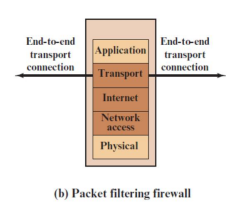
\includegraphics[width=1\textwidth]{images/chapter7/7-1.png}
    \caption{Reti wireless.}
    \label{fig:7-1}
\end{figure}

Esamina tutti i tipi di pacchetti di dati in entrata o in uscita in esecuzione sulla rete, verificando: 
\begin{itemize}
    \item Origine del pacchetto;
	\item Destinazione del pacchetto;
	\item Porta di origine e destinazione.
\end{itemize}

Quando i pacchetti superano il processo di ispezione, il firewall consente ai pacchetti di entrare nella rete o nel dispositivo. I pacchetti che non riescono a passare vengono bloccati.
Solitamente definisco le configurazioni di entrata/usciti consentite (più specifiche configurazioni non consentite) e blocco tutto il resto.

Vantaggi: semplicità, velocità, trasparente agli utenti.

Svantaggi:
\begin{itemize}
    \item Non possono impedire attacchi che impiegano vulnerabilità o funzioni delle applicazioni;  
	\item Limitate funzionalità di log (indirizzo IP, porte, tipo di traffico, flag,..);
	\item La maggior parte di questi firewall non supporta user authentication avanzate;
	\item Sono generalmente vulnerabili ad attacchi e exploit che sfruttano i problemi all'interno della specifica TCP/IP e dello stack di protocollo;
	\item Sono suscettibili a violazioni alla sicurezza causate da configurazioni improprie.
\end{itemize}

Attacchi e contromisure:
\begin{itemize}
    \item Spoofing dell'indirizzo IP: l'attaccante trasmette i pacchetti dall'esterno usando come indirizzo IP di origine l'indirizzo di un host interno (mi spaccio per un altro indirizzo IP);
	\begin{itemize}
	    \item La contromisura è scartare i pacchetti con un indirizzo di origine interno se arriva su un'interfaccia esterna (non ha senso che un pacchetto inviato da un host interno alla rete arrivi da fuori la rete). Questa contromisura è spesso implementata al router esterno al firewall.
	\end{itemize}
	\item Source routing attack: la stazione di origine specifica il percorso che un pacchetto dovrebbe seguire mentre attraversa Internet, nella speranza che ciò aggiri il firewall;
	\begin{itemize}
	    \item La contromisura consiste nell'eliminare tutti i pacchetti che lo utilizzano questa opzione.
	\end{itemize}
	\item Tiny fragment attacks: l'intruso utilizza l'opzione di frammentazione IP per creare frammenti estremamente piccoli e forzare le informazioni dell'header TCP in un frammento di pacchetto separato.
	\begin{itemize}
	    \item La contromisura consiste nell'usare una regola per cui il primo frammento di un pacchetto deve contenere una quantità minima di info sull'header del protocollo di trasporto. Se il primo frammento viene rifiutato, il filtro può ricordare il pacchetto ed eliminare tutti i frammenti successivi;
		\item Posso oppure scartare direttamente i pacchetti che usano al flag di frammentazione.
	\end{itemize}
\end{itemize}

\subsection{Firewall statefull inspection}

\begin{figure}[h]
    \centering
    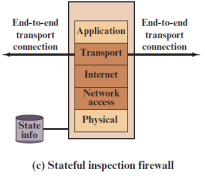
\includegraphics[width=1\textwidth]{images/chapter7/7-2.png}
    \caption{Reti wireless.}
    \label{fig:7-2}
\end{figure}

\begin{itemize}
    \item Monitora lo stato delle connessioni (tipo di connessione e porta) attive e utilizza tali informazioni per consentire ai pacchetti di rete di attraversare il firewall;
	\item L'esterno può inviare quell'informazione solo su quella connessione, quindi solo a quella porta di quell'host;
	\item Questi firewall, a volte, possono andare anche a controllare il sequence number del pacchetto TCP, per evitare attacchi di replay;
    \item Versione rinforzata dei packet-filter.
\end{itemize}

\subsection{Application-Level Gateway}

\begin{figure}[h]
    \centering
    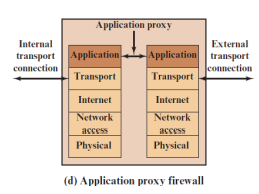
\includegraphics[width=1\textwidth]{images/chapter7/7-3.png}
    \caption{Reti wireless.}
    \label{fig:7-3}
\end{figure}

\subsection{Circuit-level gateway}

\begin{figure}[h]
    \centering
    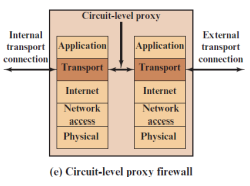
\includegraphics[width=1\textwidth]{images/chapter7/7-4.png}
    \caption{Reti wireless.}
    \label{fig:7-4}
\end{figure}

\begin{itemize}
    \item Può essere un sistema autonomo o può essere una funzione specializzata eseguita da un gateway a livello di applicazione per determinate applicazioni:
	\item Non consente una connessione TCP end to end. Si basa su due connessioni, ciascuna delle quali può avere policy diverse;
	\item La funzione di sicurezza determina quali connessioni sono consentite;
	\item Una tipica situazione d'uso è quando l'amministratore del sistema di fida degli utenti interni.
\end{itemize}

Un bastion host è un host rafforzato dal punto di vista della sicurezza (hardened OS, servizi essenziali, autenticazione rafforzata, …) che runna il circuit-level gateway ed è solitamente la prima macchina esposta su Internet.

\begin{figure}[h]
    \centering
    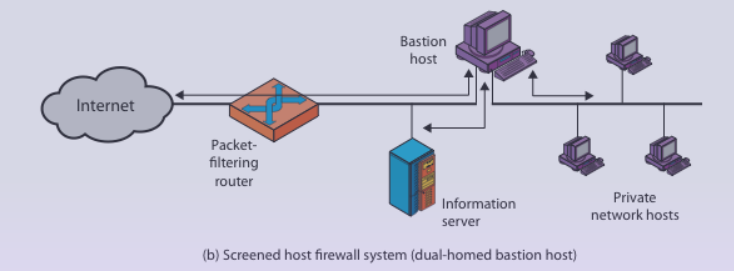
\includegraphics[width=1\textwidth]{images/chapter7/7-5.png}
    \caption{Reti wireless.}
    \label{fig:7-5}
\end{figure}

\subsection{DMZ (Demilitarised Zone)}

Si riferisce a una rete appositamente controllata situata tra la rete esterna (Internet) e la rete interna. Rappresenta una sorta di zona cuscinetto che separa le reti da rigide regole di comunicazione e firewall. L'area demilitarizzata contiene server quali server Web, server di posta, server di autenticazione o gateway applicazione. Solo questi sono accessibili agli utenti da Internet. Separando la DMZ dalla rete interna, gli utenti esterni non possono accedere alle risorse interne. La rete privata rimane protetta dagli attacchi provenienti da Internet o dal sovraccarico delle richieste Internet. La zona demilitarizzata può essere separata dalle reti adiacenti da uno o più firewall, che proteggono sia in ingresso che in uscita.

\begin{figure}[h]
    \centering
    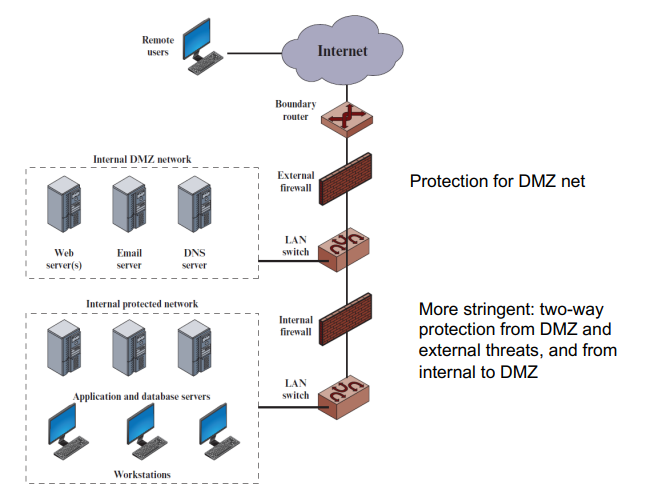
\includegraphics[width=1\textwidth]{images/chapter7/7-6.png}
    \caption{Reti wireless.}
    \label{fig:7-6}
\end{figure}

\section{Intrusion Detection System}

Concetti base:
\begin{itemize}
    \item Intrusioni: violazioni delle policy di sicurezza, generalmente caratterizzate come tentativi di intaccare la riservatezza, l'integrità o la disponibilità di un computer o di una rete. Queste violazioni possono provenire da aggressori che accedono ai sistemi da Internet o da utenti autorizzati dei sistemi che tentano di superare i loro legittimi livelli di autorizzazione o che utilizzano il loro legittimo accesso al sistema per condurre attività non autorizzate;
	\item Detection dell'intruzione: processo di raccolta delle informazioni sugli eventi che si verificano in un sistema o rete e la loro analisi alla ricerca di segni dell'intruzione;
	\item Intrusione detection system: prodotti hardware o software che raccolgono e analizzano informazioni da varie aree all'interno di un computer o una rete allo scopo di trovare e fornire avvisi in tempo reale o quasi in tempo reale di tentativi di accesso alle risorse di sistema in modo non autorizzato.
\end{itemize}

Possono essere classificati in:
\begin{itemize}
    \item Host-based IDS: monitora le caratteristiche di un singolo host e gli eventi che si verificano all'interno di tale host per attività sospette;
	\item Network-based host: monitora il traffico di rete per particolari segmenti di rete o dispositivi e analizza la rete, il trasporto e i protocolli applicativi per identificare attività sospette.
\end{itemize}

Componenti logiche:
\begin{itemize}
    \item Sensori: sono responsabili della raccolta dei dati. L'input per un sensore può essere qualsiasi parte di un sistema che potrebbe contenere prove di un'intrusione. I tipi di input per un sensore includono pacchetti di rete, file di log e tracce delle chiamate di sistema. I sensori raccolgono e inoltrano queste informazioni all'analizzatore;
	\item Analizzatore: ricevono input da uno o più sensori o da altri analizzatori. L'analizzatore è responsabile di determinare se si è verificata un'intrusione. L'output di questo componente indica che si è verificata un'intrusione. L'output può includere prove a sostegno della conclusione che si è verificata un'intrusione. L'analizzatore può fornire indicazioni sulle azioni da intraprendere a seguito dell'intrusione;
	\item Interfaccia utente: consente all'utente di visualizzare l'output del sistema o di controllare il comportamento del sistema. In alcuni sistemi, l'interfaccia utente può equivalere a un componente manager, director o console.
\end{itemize}

Approcci all'intrusion detection:
\begin{itemize}
    \item Misuse (abusi) detection: definisco delle regole di pattern di attacco. Se questi pattern si verificano allora sono sotto attacco. Ho pochi falsi positivi, ma non riconosco attacchi che non seguono i pattern che ho inserito (faccio un profilo dell'attaccante);
	\item Anomaly detection: ricerco attività anomale secondo alcuni criteri sul corretto comportamento del sistema. Può rilevare attacchi nuovi e sconosciuti, ma può generare falsi positivi/negativi (faccio un profilo sul sistema).
\end{itemize}

IDS basato su host:
\begin{itemize}
    \item Aggiunge un layer specializzato sulla sicurezza sw a sistemi vulnerabili o sensibili;
	\item Monitora le attività nel sistema in più modi per cercare comportamenti sospetti;
	\item In alcuni casi può stoppare un attacco prima che il danno venga fatto, anche se il suo compito principale resta individuare le intrusioni, loggare eventi sospetti e lanciare allarmi;
	\item Può individuare intrusioni interne e esterne;
	\item Può basarsi sulla misuse protection, anomaly protection o una combinazione di entrambe. Per l'anomaly detection, 2 strategia comuni sono:
	\begin{itemize}
	    \item Threshold detection: controllo delle soglie, come quante connessioni sto creando in parallelo, …;
		\item Profiled based: creo uno storico sul comportamento dell'utente e faccio delle stime. 
	\end{itemize}
\end{itemize}

IDS basato sulla rete (NIDS):
\begin{itemize}
    \item Monitora il traffico sul suo segmento di rete come fonte di dati, settando le interfacce delle schede di rete in modo promiscuo per catturare tutto il traffico che passa per il suo segmento di rete;
	\item Il traffico di rete sugli altri segmenti deve essere controllato da altri NIDS;
	\item Controlla i pacchetti sulla rete nel momento in cui passano per qualche sensore. Un pacchetto viene considerato se matcha una certa firma. I tipi di firma sono:
	\begin{itemize}
	    \item Stringa: cerca una strigna di testo che indica un possibile attacco;
		\item Porta: controlla tentativi di connessione a porte che sa essere attaccate frequentemente;
		\item Condizione sull'header: controlla alla ricerca di combinazioni di header illefali o pericolose.
	\end{itemize}
	\item Posso piazzare i suoi sensori in 4 punti principali della rete, per segmentarla:
	\begin{itemize}
	    \item All'ingrasso della rete;
		\item Al livello della DMZ;
		\item Al livello delle parti più importanti delle rete interna;
		\item Al livello degli host, per monitorare lo workstation.
	\end{itemize}
\end{itemize}

\begin{figure}[h]
    \centering
    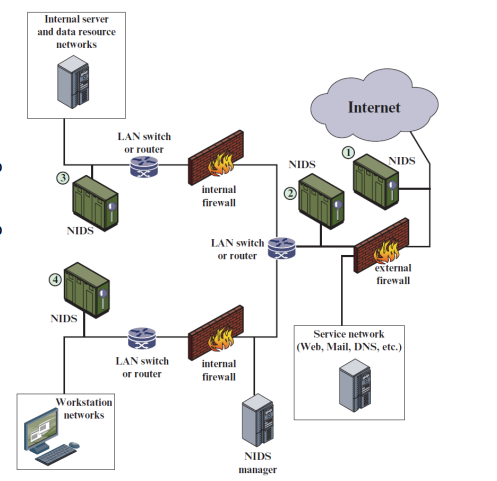
\includegraphics[width=1\textwidth]{images/chapter7/7-7.png}
    \caption{Reti wireless.}
    \label{fig:7-7}
\end{figure}
\setchapterpreamble[u]{\margintoc}
\chapter{Electronic Mail Security}
\labch{chapter8}


Tipi di protocolli usati per trasferire mail:
\begin{itemize}
    \item Per spostare i messaggi tramite Internet dalla sorgente alla destinazione: Simple Mail Transfer Protocol (SMTP);
	\item Per trasferire messaggi tra server di posta: IMAP e POP sono i più comunemente usati.
\end{itemize}

SMTP:
\begin{itemize}
    \item Protocollo client-server basato su testo;
	\item Incapsula un messaggio di posta elettronica in una busta e inoltra i messaggi incapsulati dall'origine alla destinazione tramite più MTA;
	\item Viene spesso utilizzato il termine Extended SMTP (ESMTP) per riferirsi alle versioni successive di SMTP (2008).
\end{itemize}

Protocolli di accesso alla posta:
\begin{itemize}
    \item POP3 (Post Office Protocol): 
	\begin{itemize}
	    \item Consente a un client di posta elettronica di scaricare un'email da un server di posta (MTA);
		\item Gli user agent si connettono via TCP alla porta 110 del server;
		\item \item Dopo l'autorizzazione, l'UA può usare i comandi POP3 per recuperare ed eliminare la posta.
	\end{itemize}
	\item IMAP (Internet Mail Access Protocol):
	\begin{itemize}
	    \item Consente a un client di posta elettronica di accedere alla posta su un server email;
		\item Usa TCP sulla porta 143;
		\item È più complesso di POP3;
		\item Fornisce un'autenticazione più forte e funzioni non supportate da POP3.
	\end{itemize}
\end{itemize}

\subsection{RFC 5322}

Definisce un formato per i messaggi di testo inviati utilizzando email. I messaggi sono visti come una busta più un contenuto:
\begin{itemize}
    \item La busta contiene tutte le informazioni necessarie per effettuare la trasmissione e la consegna;
	\item Il contenuto compone l'oggetto da consegnare al destinatario;
	\item Lo standard RFC 5322 si applica solo ai contenuti;
	\item Lo standard del contenuto include una serie di campi di intestazione che possono essere utilizzati dal sistema di posta per creare la busta.
\end{itemize}

Lo schema SMTP/5322 ha pensanti limiti:
\begin{itemize}
    \item SMTP non può trasmettere file eseguibili o altri oggetti binari;
	\item SMTP non può trasmettere dati di testo che includono caratteri della lingua nazionale;
	\item I server SMTP possono rifiutare i messaggi di posta di una certa dimensione;
	\item I gateway SMTP che si occupano della traduzione da ASCII al codice carattere EBCDIC non utilizzano un insieme coerente di mappature, con conseguenti problemi di traduzione;
	\item Alcune implementazioni SMTP non aderiscono completamente agli standard.
\end{itemize}


\subsection{Multipurpose Internet Mail Extension (MIME)}

Estensione al framework RFC 5322 che ha lo scopo di affrontare alcuni dei problemi e delle limitazioni di SMTP. La specifica MIME include i seguenti elementi:
\begin{itemize}
    \item Vengono definiti cinque nuovi campi di intestazione del messaggio, che possono essere inclusi in un Intestazione RFC 5322. Questi campi forniscono informazioni sul corpo del messaggio;
	\item Vengono definiti diversi formati di contenuto, standardizzando così le rappresentazioni che supportano la posta elettronica multimediale;
	\item Sono definite codifiche di trasferimento che consentono la conversione di qualsiasi formato di contenuto in un modulo protetto da alterazioni al sistema di posta.
\end{itemize}

I cinque campi di intestazione definiti in MIME sono:
\begin{itemize}
    \item Versione MIME: Deve avere valore 1.0, per indicare che il messaggio è conforme a RFC 2045 e 2046;
	\item Tipo di contenuto: descrive i dati contenuti nel corpo con dettagli sufficienti affinché l'agent user ricevente possa scegliere un agente o un meccanismo appropriato per rappresentare i dati per l'utente o altrimenti trattare i dati in modo appropriato;
	\item Codifica di trasferimento dei dati: indica il tipo di trasformazione che è stata utilizzata per rappresentare il corpo del messaggio in un modo accettabile per il trasporto della posta;
	\item Content ID: Utilizzato per identificare le entità MIME in modo univoco in più contesti;
	\item Descrizione del contenuto: descrizione testuale dell'oggetto con il corpo (questo è utile quando l'oggetto non è leggibile).
\end{itemize}

Codifiche dei dati:
\begin{itemize}
    \item 7 bit: i dati sono tutti rappresentati da brevi righe di caratteri ASCII;
    \item 8 bit: le righe sono brevi, ma potrebbero essere presenti caratteri non ASCII;
    \item Binario: non solo possono essere presenti caratteri non ASCII, ma le righe non sono necessariamente sufficientemente corte per il trasporto SMTP;
    \item Quoted-printable: utile quando i dati sono costituiti da testo ASCII, la codifica è ampiamente riconoscibile dagli esseri umani;
    \item Base64: comunemente usato per codificare dati binari arbitrari in modo che non vengano modificati dal programma di mail-transport;
    \item x-token: codifica non standard
\end{itemize}

Nei primi tre casi non viene effettuata alcuna codifica. Il campo in questo caso serve solo per specificare info sulla natura del dato.

Un concetto importante in MIME e S/MIME è quello di forma canonica. La forma canonica è un formato, appropriato al tipo di contenuto, standardizzato per l'uso tra i sistemi. Ciò è in contrasto con la forma nativa, che è un formato che può essere peculiare di un particolare sistema.

\section{Email security}

Le mail sono soggette a più minacce:
\begin{itemize}
    \item Minacce relative all'autenticità: accesso non autorizzato al sistema di posta elettronica di un'azienda;
	\item Minacce legate all'integrità: modifica non autorizzata del contenuto dell'e-mail;
	\item Minacce legate alla riservatezza: divulgazione non autorizzata di informazioni sensibili;
	\item Minacce relative alla disponibilità: impedimento agli utenti finali di inviare o ricevere posta.
\end{itemize}

Protocolli contro le minacce

I protocolli standardizzati per contrastare le minacce sono:
\begin{itemize}
    \item STARTTLS: estensione di sicurezza di SMPT che fornisce autenticazione, integrità, non ripudiabilità e riservatezza per l'intero messaggio SMTP eseguendo SMTP su TLS;
	\item S/MIME: fornisce autenticazione, integrità, non ripudiabilità e riservatezza del corpo del messaggio trasportato in messaggi SMTP;
	\item DNSSEC (DNS security extention): fornisce autenticazione e protezione dell'integrità dei dati DNS ed è uno strumento utilizzato da vari protocolli di sicurezza della posta elettronica;
	\item DAME (DNS-based Authentication of Named Entities): progettato per superare problemi nel sistema delle CA fornendo un canale alternativo per l'autenticazione delle chiavi pubbliche basate su DNSSEC, con il risultato che le stesse relazioni di fiducia utilizzate per certificare gli indirizzi IP vengono utilizzate per certificare i server che operano su tali indirizzi.
\end{itemize}

\subsection{S/MIME}

Miglioramento della sicurezza dello standard MIME basato sulla tecnologia di RSA Data Security.
I servizi che offre sono:
\begin{itemize}
    \item Firma digitale con RSA/SHA-256;
	\item Cifratura dei messaggi con AES-128 con block chain;
	\item Compressione;
	\item Compatibilità email.
\end{itemize}

Autenticazione: fornita tramite firma digitale. Passi:
\begin{itemize}
    \item Il mittente crea il messaggio;
	\item Viene usato SHA-256 (one-way function) per creare un messaggio digest di 256 bit;
	\item Il digest viene cifrato con RSA utilizzando la chiave privata del mittente e il risultato viene aggiunto al messaggio. Vengono inoltre aggiunte le informazioni di identificazione per il firmatario, che consentiranno al destinatario di recuperare la chiave pubblica del firmatario;
	\item Il destinatario utilizza RSA con la chiave pubblica del mittente per decrittografare e recuperare il digest del messaggio;
	\item Il destinatario calcola il digest del messaggio per il messaggio e lo confronta con il codice hash decrittografato. Se i due corrispondono, il messaggio viene accettato come autentico.
\end{itemize}

Vengono accettate anche firme inviate separate dal messaggio che firmano. Queste possono essere usate per effettuare controlli successivi sul messaggio (es: rilevare successivamente se il programma è stato infettato da virus).

Confidenzialità: garantita cifrando i messaggi con AES con una chiave a 128 bit, con la modalità Cipher Block Chaining (CBC). Anche la chiave stessa è crittografata, in genere con RSA (quindi meccanismo chiave pubblica). Ciascuna chiave simmetrica viene utilizzata una sola volta:
\begin{itemize}
    \item Viene generata una nuova chiave come numero casuale per ciascun messaggio;
	\item Poiché deve essere utilizzata una sola volta, la chiave è vincolata al messaggio e trasmessa con esso;
	\item Per ridurre i tempi di crittografia, viene utilizzata la combinazione di crittografia simmetrica (per il contenuto del messaggio) e a chiave pubblica (per la chiave);
	\item Solo il destinatario è in grado di recuperare la chiave contenuta nel messaggio, in quanto è necessaria la sua chiave private per decifrarla.
\end{itemize}
	
Compatibilità mail: molti sistemi di posta elettronica consentono solo l'uso di blocchi che contengono testo ASCII. Per soddisfare questa restrizione, S/MIME fornisce il servizio di conversione.

Compressione: la compressione, opzionale, permette di risparmiare spazio sia per la trasmissione di mail che per lo storage dei file. La compressione può essere applicata in qualsiasi ordine rispetto alle operazioni di firma e crittografia dei messaggi. 

S/MIME usa i seguenti content type:
\begin{itemize}
    \item Dati (questo si riferisce ai tipi di contenuto del messaggio di MIME): si riferisce al contenuto gestito da MIME, che potrebbe poi essere incapsulato in un tipo SignedData, EnvelopedData o CompressedData;
	\item SignedData: usato per applicare la firma digitale al messaggio, contiene le info relative alla firma. Passi:
	\begin{itemize}
	    \item Seleziono un algoritmo di digest del messaggio (SHA o MD5 -> MD5 è sconsigliato);
		\item Calcolo il message digest (funzione hash) del contenuto da firmare;
		\item Cifro il digest con la chiave privata del firmatario;
		\item Preparo un blocco con le info per calcolare e confrontare il digest.
	\end{itemize}
	\item EnvelopedData: contiene i dati cifrati e le chiavi di cifratura. Passi:
	\begin{itemize}
	    \item Genero la chiave di sessioni con funzione pseudorandom per l'algoritmo di cifratura;
		\item Cifro la chiave di sessione con la chiave pubblica del destinatario;
		\item Preparo un blocco con le info necessarie al destinatario per decifrare;
		\item Cifro il messaggio.
	\end{itemize}
	\item CompressedData: usato per applicare compressione al messaggio.
\end{itemize}

Sicurezza di un'entità MIME:
\begin{itemize}
    \item S/MIME protegge un'entità MIME con una firma, una crittografia o entrambe;
	\item All'entità protetta vengono poi aggiunte una serie di info relative alla sicurezza, come certificati e ID degli algoritmi usati;
	\item Il tutto viene processato in un oggetto PKCS, che viene considerato come il contenuto del messaggio e wrappato in MIME.
\end{itemize}

Gestione dei certificati in S/MIME:
\begin{itemize}
    \item S/MIME utilizza certificati conformi alla versione 3 di X.509;
	\item I gestori e/o gli utenti S/MIME devono configurare ogni client con un elenco di chiavi attendibili e con elenchi di revoche di certificati. La responsabilità è locale per il mantenimento dei certificati necessari per verificare le firme in entrata e per crittografare i messaggi in uscita;
\end{itemize}

Gli user-agent di S/MIME svolgono una serie di funzioni legate alle chiavi:
\begin{itemize}
    \item Generazione delle chiavi;
	\item Registrazione: La chiave pubblica di un utente deve essere registrata con una autorità di certificazione per ricevere un certificato di chiave pubblica X.509;
	\item Archivio e recupero dei certificati.
\end{itemize}

RFC 2634 definisce una serie di servizi di sicurezza migliorati per S/MIME:
\begin{itemize}
    \item Signed receipt: la restituzione di una ricevuta firmata fornisce la prova della consegna al mittente del messaggio e gli consente di dimostrare a una terza parte che il destinatario ha ricevuto il messaggio;
	\item Security labels: insieme di informazioni di sicurezza relative alla sensibilità del contenuto protetto dall'incapsulamento S/MIME. Può essere utilizzato per il controllo degli accessi o determinarne la priorità;
	\item Secure mailing lists: ricevo un singolo messaggi, eseguire la crittografia specifica per ciascun membro della lista e lo inoltro a ogni destinatario;
	\item Signing certificates: questo servizio viene utilizzato per vincolare in modo sicuro il certificato del mittente alla propria firma tramite un attributo specifico.
\end{itemize}

\subsection{DNSSEC}

DNS (Domain Name System) è un servizio di ricerca che fornisce una mappatura tra il nome di un host su Internet e il suo indirizzo IP. Si compone di quattro elementi:
\begin{itemize}
    \item Domain Name Space: uno spazio dei nomi con struttura ad albero per identificare le risorse della rete;
	\item Database DNS: DB gerarchico costituito da record di risorse (RR) contenenti nomi, indirizzi IP, …;
	\item Name server: server che contengono informazioni su DNS e RR;
	\item Risolutori: programmi che estraggono informazioni dai name server per risolvere le richieste dei client.
\end{itemize}

Il DNS si basa su un database gerarchico contenente record di risorse (RR) che includono il nome, l'indirizzo IP e altre informazioni sugli host. Le caratteristiche principali del DATABASE DNS sono:
\begin{itemize}
    \item Gerarchia a profondità variabile per i nomi: consente un livello illimitato separato da ".";
	\item Database distribuito: esistono più server DNS sparsi in Internet;
	\item Distribuzione controllata dal database: il database è suddiviso in molteplici zone.
\end{itemize}

Esempio di risoluzione di un nome:
\begin{enumerate}
    \item Il programma utente richiede l'indirizzo IP per il nome del server;
	\item Il risolutore tenta di risolvere con i dati nella sua cache, altrimenti l'ISP interroga un server dei nomi locale;
	\item L'ISP trova l'indirizzo IP nel suo database locale o interroga altri server dei nomi;
	\item Quando la risposta viene ricevuta nel locale name server è memorizzato nella cache;
	\item Il programma utente riceve un indirizzo IP o un messaggio di errore.
\end{enumerate}

DNSSEC: 
\begin{itemize}
    \item Estensione con sicurezza di DNS;
	\item Fornisce protezione end-to-end tramite l'uso di firme digitali create dagli amministratori di zona e verificate dal software di risoluzione del destinatario;
	\item Evita la necessità di considerare attendibili server dei nomi e risolutori intermedi. Si crea infatti una catena di trust tra gli zone administrator, ciascuno dei quali garantisce per la propria zona;
	\item Consiste in un insieme di nuovi tipi di record di risorse e modifiche al protocollo DNS esistente;
\end{itemize}
	
In sostanza, DNSSEC è progettato per proteggere i client DNS dall'accettazione di record di risorse DNS contraffatti o alterati. Lo fa utilizzando le firme digitali per fornire:
\begin{itemize}
    \item Autenticazione dell'origine dei dati: garantisce che i dati provengano dalla fonte corretta (amministratore della zona DNS);
	\item Verifica dell'integrità dei dati: garantisce che il contenuto di un record di risorse (RR) non sia stato modificato.
\end{itemize}

La fiducia nella chiave pubblica della sorgente (dell'amministratore della zona DNS) è stabilita partendo da una zona di fiducia e stabilendo la catena di fiducia fino all'attuale fonte di risposta attraverso successive verifiche di firma della chiave pubblica di un figlio da parte del suo genitore. La chiave pubblica di una zona trusted è chiamata anchor trust.

DNSSEC aggiunge una serie di nuovi campi ai record di risorse (RR), per info sulle firme o per dire che quel name server non è parte di una determinata zona fornendo la lista di nomi del DNS (NSEC).
DNSSEC si basa sullo stabilire l'autenticità della gerarchia NDS che porta al domain name che mi interessa, e quindi dipende dalla root da cui inizio. La catena di autenticazione che va dalla mia root fino al domain name viene creata tramite autenticazione tra zone DNS. Per proteggere tutte le ricerche DNS, comprese quelle per nomi di dominio e tipi di record inesistenti, DNSSEC utilizza il record di risorse NSEC per autenticare le risposte negative alle query (serve per autenticare che la risposta "il domain name non esiste" arriva effettivamente dal server).

\subsection{DANE}

Protocollo che consente ai certificati X.509, comunemente usati in TLS, di essere associati ai nomi DNS tramite DNSSEC. Viene proposto come un modo per autenticare client e server TLS senza una CA. Lo scopo di DANE è sostituire l'affidarsi alla sicurezza del sistema delle CA con quello di DNSSEC.

DANE definisce un nuovo tipo di record DNS, TLSA, che può essere usato come metodo sicuro per autenticare certificati SSL/TLS. Questo record vincola l'emissione e la consegna del certificato a un dato dominio:
\begin{itemize}
    \item Il proprietario del dominio del server crea il record TLSA che identifica il certificato;
	\item Quando il client riceve il certificato, cerca il relativo record TLSA per quel dominio e confronta i dati del record con il certificato.
\end{itemize}

Poco diffuso.

\section{Sender Policy Framework (SPF)}

SPF è il metodo standardizzato per validare se il mittente della mail è autorizzato ad usare quello specifico dominio (permette di identificare mail forgiate, sta alla base del sistema di spam). 
Funzionamento:
\begin{itemize}
    \item Il proprietario di un dominio specifica la propria policy di invio della posta (es: quali server di posta utilizzano per inviare posta dal loro dominio);
	\item Il proprietario del dominio pubblica queste informazioni in un record SPF nella zona DNS del dominio;
	\item Quando il server di posta di qualcun altro riceve un messaggio che afferma di provenire da quel dominio, il server ricevente può verificare se il messaggio è conforme alla policy dichiarata del dominio (es: se il messaggio proviene da un server sconosciuto, può essere considerato un falso).
\end{itemize}

I record SPF vengono controllati nel momento in cui accedo al DNS.

\begin{figure}[h]
    \centering
    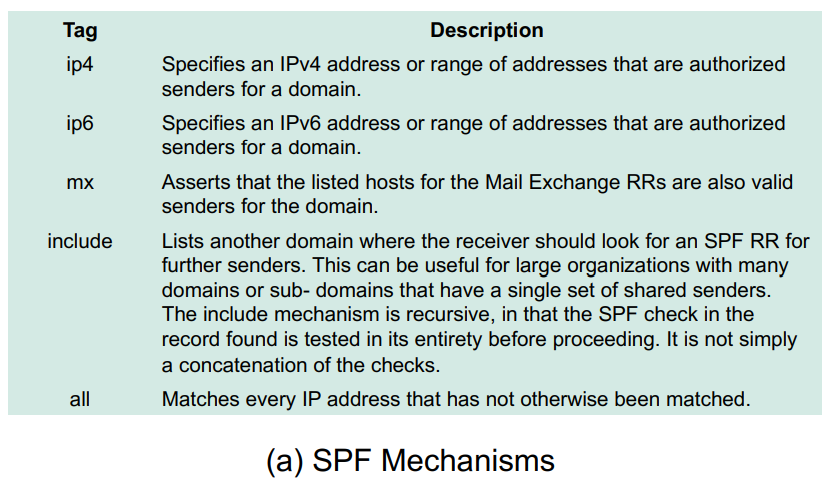
\includegraphics[width=1\textwidth]{images/chapter8/8-1.png}
    \caption{Reti wireless.}
    \label{fig:8-1}
\end{figure}

\begin{figure}[h]
    \centering
    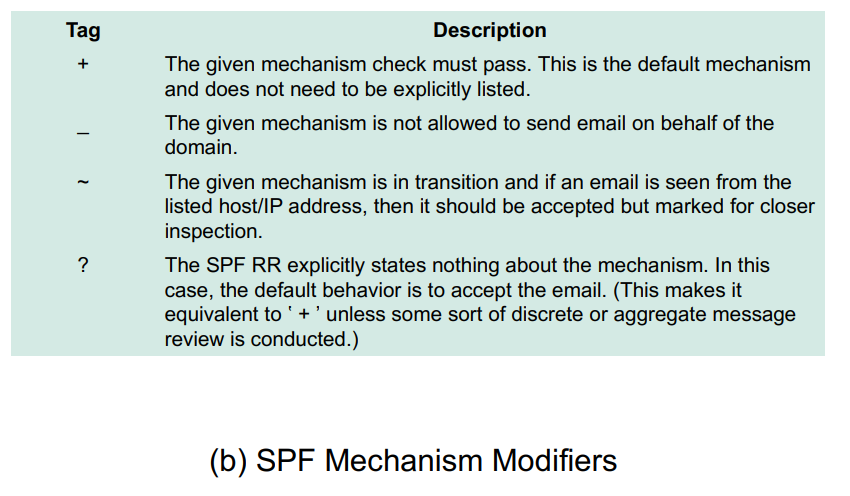
\includegraphics[width=1\textwidth]{images/chapter8/8-2.png}
    \caption{Reti wireless.}
    \label{fig:8-2}
\end{figure}

\section{DomainKeys Identified Mail (DKIM)}

Specifica per la firma crittografica dei messaggi di posta elettronica, che consente a un dominio di firma di rivendicare la responsabilità di un messaggio nel flusso di posta. Sostanzialmente permette ai responmsabili del dominio di garantire la validutà della mail (es: gmail garantisce la validità della mail). I destinatari del messaggio possono verificare la firma interrogando direttamente il dominio del firmatario per recuperare la chiave pubblica appropriata e possono così confermare che il messaggio è stato attestato da un soggetto in possesso della chiave privata del dominio di firma. È stato ampiamente adottato da una serie di provider di posta elettronica e ISP (gmail, yahoo, ecc.) .

Strategia:
\begin{itemize}
    \item DKIM fornisce una tecnica di autenticazione e-mail trasparente per l'utente finale;
	\item Il messaggio di posta elettronica di un utente è firmato da una chiave privata del dominio amministrativo da cui ha origine l'e-mail;
	\item La firma copre tutto il contenuto del messaggio e parte dell'header;
	\item Il ricevente può accedere alla chiave pubblica corrispondente tramite un DNS e verificare la firma, autenticando così che il messaggio provenga dal dominio amministrativo rivendicato. 
	\item Questo approccio è diverso da quello di S/MIME, che utilizza la chiave privata del mittente per firmare il contenuto del messaggio.
\end{itemize}

\section{Domain-Based Message Authentication, Reporting, and Conformance (DMARC)}

Consente ai mittenti di posta elettronica di specificare la politica su come gestire la posta, i tipi di rapporti che i destinatari possono inviare e la frequenza con cui tali rapporti dovrebbero essere inviati.

DMARC funziona con SPF e DKIM:
\begin{itemize}
    \item SPF e DKIM consentono ai mittenti di avvisare i destinatari, tramite DNS, se una mail del mittente è valida e se deve essere consegnata, contrassegnata o eliminata;
	\item Né SPF né DKIM includono un meccanismo per dire ai ricevitori se essi sono in uso, né dispongono di meccanismi di feedback per informare i mittenti dell'efficacia delle tecniche anti-spam;
\end{itemize}

DMARC risolve questi problemi essenzialmente standardizzando il modo in cui i ricevitori di posta elettronica eseguono l'autenticazione e-mail utilizzando i meccanismi SPF e DKIM


\setchapterpreamble[u]{\margintoc}
\chapter{IP security}
\labch{chapter9}

Perché IPsec:
\begin{itemize}
    \item Il protocollo Internet (IP) non è sicuro:  è stato progettato nelle prime fasi di Internet in cui  la sicurezza non era un problema. Non garantisce integrità o riservatezza dei dati, è soggetto a replay di pacchetti e spoofing della fonte;
	\item IPsec fornisce un canale sicuro per tutte le applicazioni (cifratura e autenticazione del traffico);
	\item IPsec permette di fare un filtraggio basato su policy;
	\item È installato nei pc (per garantire sicurezza end-to-end) e gateway (firewall, router).
\end{itemize}

IPsec garantisce:
\begin{itemize}
    \item Riservatezza, cifrando i dati;
	\item Integrità, verificata dai router calcolando l'hash o il checksum del messaggio;
	\item Autenticazione, tramite firme e certificati.
\end{itemize}

Overview sulla sicurezza IP, RFC 1636:
\begin{itemize}
    \item Identifica le aree chiave per i meccanismi di sicurezza:
	\begin{itemize}
	    \item Necessità di proteggere l'infrastruttura di rete da monitoraggio e controllo non autorizzati del traffico di rete;
		\item Necessità di proteggere il traffico da utente finale a utente finale utilizzando meccanismi di autenticazione e crittografia.
	\end{itemize}
	\item Includeva l'autenticazione e la crittografia come funzionalità di sicurezza necessarie nell'IP di prossima generazione (IPv6). Ora la specifica IPsec esiste come un insieme di standard di Internet.
\end{itemize}

 Documenti di IPsec:
\begin{itemize}
    \item Architettura: copre i concetti generali, i requisiti di sicurezza, le definizioni e i meccanismi che definiscono la tecnologia IPsec;
	\item Authentication header (AS): estensione dell'header che permette di fornire autenticazione al messaggio.
	\item Encapsulation Security Payload Header (ESP): consiste di un header e un trailer (rimorchio) di incapsulazione che forniscono crittografia o una combinazione di crittografia e autenticazione;
	\item Internet Key Exchange (IKE): raccolta di documenti che descrivono gli schemi di gestione delle chiavi da utilizzare con IPsec;
	\item Algoritmi crittografici: comprende un ampio insieme di documenti che definiscono algoritmi crittografici per la crittografia, l'autenticazione dei messaggi, le funzioni pseudocasuali (PRF) e lo scambio di chiavi crittografiche;
	\item Altro: esistono numerose altre RFC relative a IPsec, tra cui quelli che si occupano della security policy.
\end{itemize}

Applicazioni di IPsec:
\begin{itemize}
    \item IPsec offre la capacità di proteggere le comunicazioni in LAN, WAN reti pubbliche e private, Internet, come:
	\begin{itemize}
	    \item Connettività sicura delle filiali su Internet (VPN su Internet o WAN pubblica);
		\item Accesso remoto sicuro su Internet (chiamata locale sicura all'ISP);
		\item Stabilire connettività Extranet e Intranet con i partner (comunicazioni sicure con altre organizzazioni);
		\item Miglioramento della sicurezza del commercio elettronico.
	\end{itemize}
	\item La caratteristica principale di IPsec è che può crittografare e/o autenticare tutto il traffico a livello IP. In questo modo tutte le applicazioni distribuite (accesso remoto, client/server, e-mail, trasferimento file, accesso Web) possono essere protette.
\end{itemize}

IPsec fornisce una serie di opzioni da scegliere per fare un'associazione di sicurezza tra due macchine:
\begin{itemize}
    \item IPsec fornisce servizi di sicurezza a livello IP consentendo a un sistema di: 
	\begin{itemize}
	    \item Selezionare i protocolli di sicurezza richiesti ;
		\item Determinare gli algoritmi da utilizzare per i servizi;
		\item Prepara le chiavi necessarie per i servizi richiesti;
	\end{itemize}
	\item RFC 4301 elenca i seguenti servizi:
	\begin{itemize}
	    \item Controllo degli accessi;
		\item Integrità senza connessione;
		\item Autenticazione sull'origine dei dati;
		\item Rifiuto dei pacchetti riprodotti/replayed (una forma di integrità parziale della sequenza);
		\item Riservatezza, tramite crittografia;
		\item Cerca di ridurre l'analisi sul traffico.
	\end{itemize}
\end{itemize}

\section{Architettura IP}

\begin{figure}[h]
    \centering
    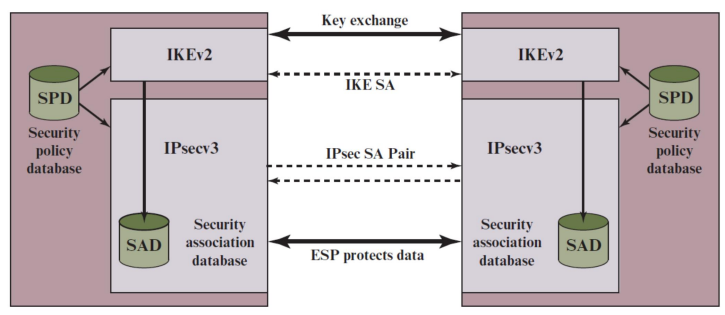
\includegraphics[width=1\textwidth]{images/chapter9/9-1.png}
    \caption{Reti wireless.}
    \label{fig:9-1}
\end{figure}

La politica IPsec è determinata dall'interazione di due database: il database dell'associazione di sicurezza (SAD) e il database della politica di sicurezza (SPD)

Security Association (SA):
\begin{itemize}
    \item Connessione logica unidirezionale tra un mittente e un destinatario che offre servizi di sicurezza sul traffico che trasporta;
	\item Nel senso inverso l'associazione di sicurezza potrebbe essere diversa;
	\item In qualsiasi pacchetto IP, la SA è identificata in modo univoco dall'indirizzo di destinazione nell'header IP e dall'SPI presente nell'estensione dell'header (AH o ESP).
\end{itemize}

Un'associazione di sicurezza è identificata da 3 parametri:
\begin{enumerate}
    \item Security Parameter Index (SPI): intero senza segno a 32 bit usatp per identificare in modo univoco questo SA e con significato solo locale (trasportato nell'intestazione IPsec: AH o ESP);
	\item Indirizzo IP di destinazione: indirizzo dell'endpoint di destinazione della SA, che può essere un sistema dell'utente finale o un sistema di rete come un firewall o un router;
	\item Identificatore del protocollo di sicurezza: indica se l'associazione è un'associazione di sicurezza AH o ESP.
\end{enumerate}

Security Association Database (SAD):
\begin{itemize}
    \item Definisce i parametri associati a ciascuna SA;
	\item Normalmente definito dai seguenti parametri in una entry SAD: 
	\begin{itemize}
	    \item Indice del parametro di sicurezza;
		\item Contatore del numero di sequenza (info sui pacchetti che seguono che hanno quell'associazione di sicurezza);
		\item Overflow del contatore di sequenza (per impedire ulteriori trasmissioni di pacchetti);
		\item Finestra anti-replay (per determinare se un pacchetto AH o ESP in entrata è un replay);
		\item Informazioni AH (algoritmo di autenticazione, chiavi, durata delle chiavi, parametro utilizzato con AH);
		\item Informazioni ESP (encr./auth. Algorithms, keys, init. values, key lives, param. ESP);
		\item Durata di questa associazione di sicurezza;
		\item Modalità del protocollo IPsec (tunnel, trasporto, wildcard);
		\item Path MTU (dimensione massima di un pacchetto che può essere trasmessa senza frammentazione).
	\end{itemize}
\end{itemize}

Security Policy Database (SPD):
\begin{itemize}
    \item Specifica le modalità attraverso le quali il traffico IP è correlato a specifiche SA. Contiene una serie di entry, ognuna delle quali definisce un sottoinsieme di traffico IP e punta a una SA per quel traffico;
	\item In ambienti più complessi, potrebbero esserci più voci che potenzialmente si riferiscono a una singola SA o a più SA associate a una singola voce SPD:
	\begin{itemize}
	    \item Ciascuna entry SPD è definita da una serie di valori di campo del protocollo IP e di livello superiore chiamati selettori;
		\item Questi sono utilizzati per filtrare il traffico in uscita al fine di mapparlo in una particolare SA.
	\end{itemize}
\end{itemize}

Una entry SPD è formata come segue:
\begin{itemize}
    \item Indirizzo IP remoto: può essere un singolo indirizzo IP, un elenco enumerato o un intervallo di indirizzi o una maschera. Gli ultimi due sono necessari per supportare più di un sistema di destinazione che condivide la stessa SA;
	\item Indirizzo IP locale: può essere un singolo indirizzo IP, un elenco enumerato o un intervallo di indirizzi o una maschera. Gli ultimi due sono richiesti per supportare più di un sistema sorgente che condivide la stessa SA;
	\item Protocollo del livello superiore: l'intestazione del protocollo IP include un campo che designa il protocollo operante su IP (TCP, UDP);
	\item Nome: un identificatore utente dal sistema operativo. Non è un campo nell'header di IP o dei protocolli superiori, ma è disponibile se IPsec è in esecuzione sullo stesso sistema operativo dell'utente;
	\item Porte locali e remote: possono essere valori di singole porte TCP o UDP, un elenco enumerato di porte o una porta con caratteri jolly.
\end{itemize}

\begin{figure}[h]
    \centering
    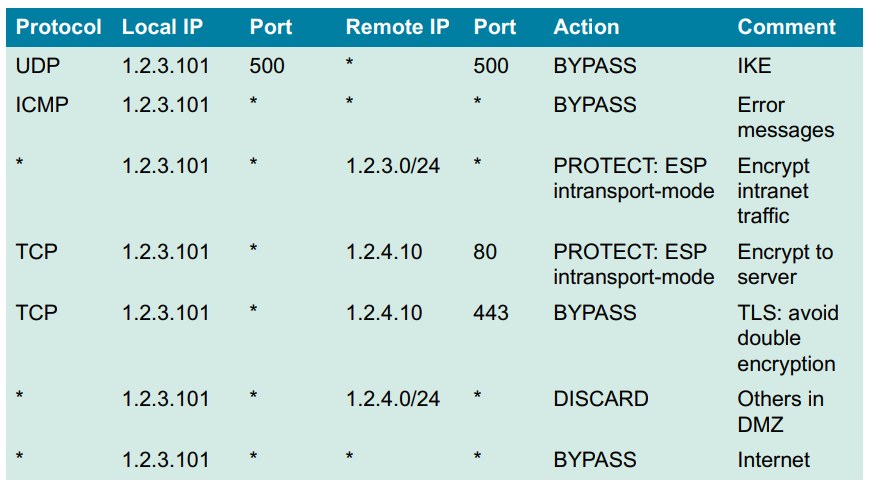
\includegraphics[width=1\textwidth]{images/chapter9/9-2.png}
    \caption{Reti wireless.}
    \label{fig:9-2}
\end{figure}

\subsection{Flow per pacchetti in entrata}

\begin{figure}[h]
    \centering
    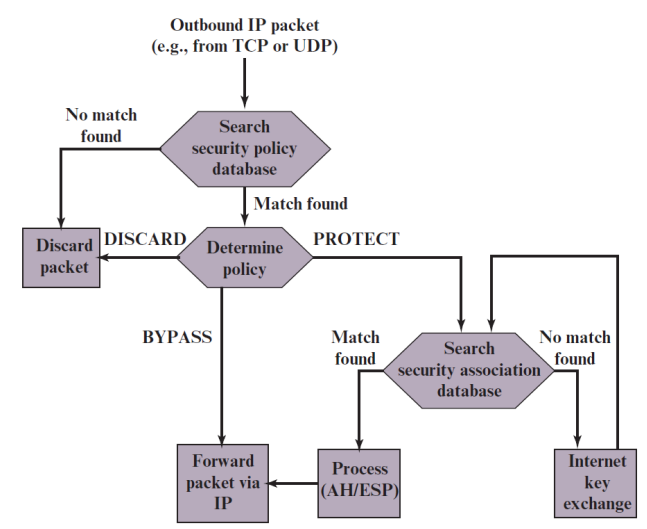
\includegraphics[width=1\textwidth]{images/chapter9/9-3.png}
    \caption{Reti wireless.}
    \label{fig:9-3}
\end{figure}

\subsection{Flow per pacchetti in uscita}

\begin{figure}[h]
    \centering
    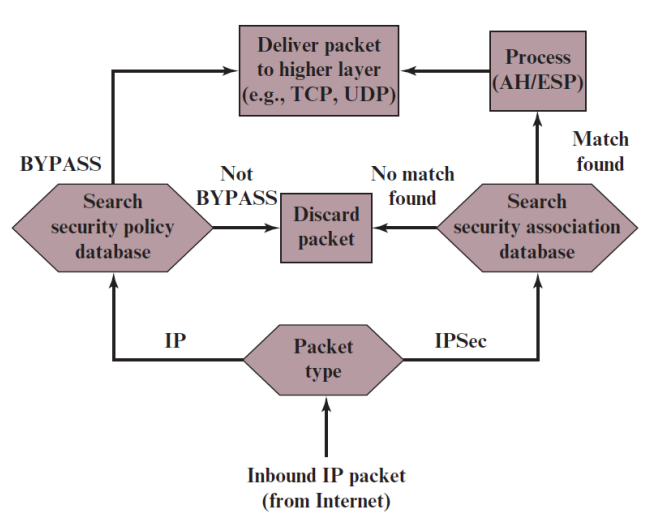
\includegraphics[width=1\textwidth]{images/chapter9/9-4.png}
    \caption{Reti wireless.}
    \label{fig:9-4}
\end{figure}

\section{Modalità di IPsec}

L'header di IPsec può essere AH o ESP.

Modalità Tunnel:
\begin{itemize}
    \item L'intero pacchetto IP viene crittografato e diventa il componente di dati di un nuovo (e più grande) pacchetto IP (il routing cambia);
	\item Utilizzato frequentemente in una VPN IPsec da sito a sito.
\end{itemize}

Modalità di trasporto:
\begin{itemize}
    \item L'header di IPsec viene inserito nel pacchetto IP (il routing rimane intatto);
	\item Non viene creato nessun nuovo pacchetto (l'header di AH assicura che gli indirizzi IP restino invariati);
	\item Funziona bene in reti in cui aumentare la dimensione del pacchetto causerebbe problemi;
	\item Utilizzato frequentemente per VPN ad accesso remoto (originariamente introdotte per permettere ai lavoratori da qualunque luogo del modo di connettersi in modo sicuro alla rete aziendale).
\end{itemize}

\begin{figure}[h]
    \centering
    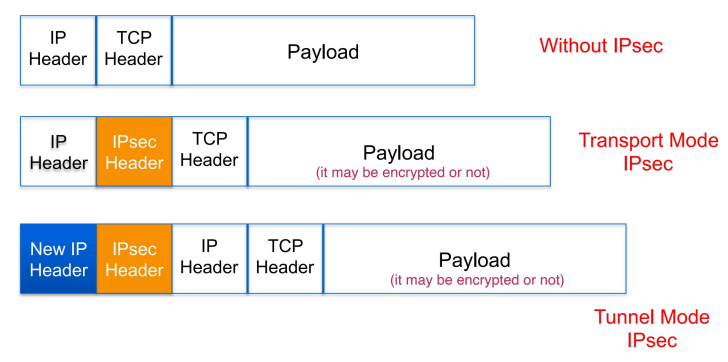
\includegraphics[width=1\textwidth]{images/chapter9/9-5.png}
    \caption{Reti wireless.}
    \label{fig:9-5}
\end{figure}

\subsection{Autentication Header (AH)}

Caratteristiche:
\begin{itemize}
    \item Header aggiuntivo tra i livelli 3 e 4 (TCP e IP) che fornisce informazioni sufficienti alla destinazione per identificare SA;
	\item AH garantisce solo l'integrità, ma protegge anche parte dell'intestazione IP;
    \item Il numero di sequenza viene inizializzato a zero e incrementato dal mittente per ogni pacchetto. Il ricevitore memorizza i pacchetti in arrivo in una finestra scorrevole (dimensione predefinita 64) per ordinare e individuare i duplicati. (IP non garantisce la consegna o l'ordine).
\end{itemize}

\begin{figure}[h]
    \centering
    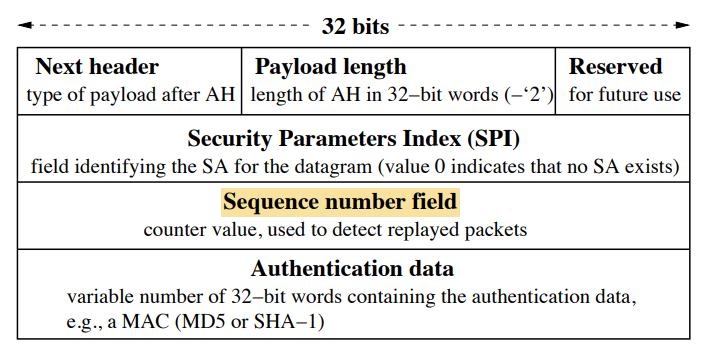
\includegraphics[width=1\textwidth]{images/chapter9/9-6.png}
    \caption{Reti wireless.}
    \label{fig:9-6}
\end{figure}

Nello specifico AH:
\begin{itemize}
    \item Per la modalità di trasporto inserisce:
	\begin{itemize}
	    \item L'intestazione IP, prima del payload IP;
		\item MAC calcolato sull'intero pacchetto (tranne che per i campi mutabili);
		\item  Fornisce protezione end-to-end tra i sistemi abilitati IPsec. 
	\end{itemize}
	\item Per la modalità tunnel:
	\begin{itemize}
	    \item L'intero pacchetto originale viene autenticato;
		\item Viene aggiunta un nuovo header IP esterno;
		\item L'header interno contiene l'indirizzo di origine/destinazione definitivo;
		\item Anche il nuovo header esterno è protetto (tranne i campi modificabili) e può contenere diversi indirizzi IP, ad esempio firewall o gateway di sicurezza.
	\end{itemize}
\end{itemize}

AH è utilizzato per fornire canali autenticati end-to-end (in genere modalità di trasporto) o nel modello di tunnel a un gateway di sicurezza.

\begin{figure}[h]
    \centering
    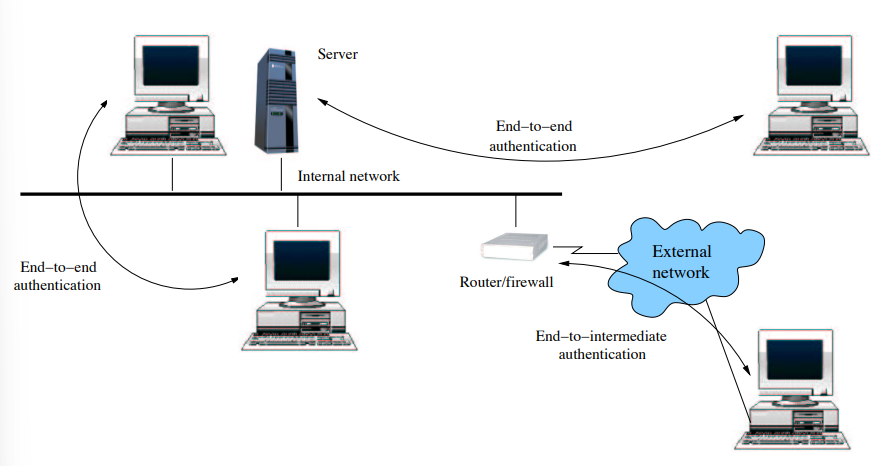
\includegraphics[width=1\textwidth]{images/chapter9/9-7.png}
    \caption{Reti wireless.}
    \label{fig:9-7}
\end{figure}

\subsection{Encapsulation Security Payload (ESP)}

Caratteristiche:
\begin{itemize}
    \item Utilizzato per crittografarei campi di payload, padding, lunghezza del padding e next header;
	\item Se l'algoritmo richiede dati di sincronizzazione per la crittografia, questi possono essere trasportati esplicitamente all'inizio del payload;
	\item Un campo ICV facoltativo è presente solo se il servizio di integrità è selezionato e fornito da un algoritmo di integrità separato o da un algoritmo in modalità combinata che utilizza un ICV:
	\begin{itemize}
	    \item L'ICV viene calcolato dopo l'esecuzione della crittografia;
		\item Questo ordine di elaborazione facilita la riduzione dell'impatto di attacchi DDoS;
		\item Poiché l'ICV non è protetto dalla crittografia, è necessario utilizzare un algoritmo di integrità con chiave per calcolare l'ICV;
	\end{itemize}
	\item Il campo relativo al padding ha più scopi:
	\begin{itemize}
	    \item Se un algoritmo di crittografia richiede che il testo in chiaro sia un multiplo di un certo numero di byte, il campo Padding viene utilizzato per espandere il testo in chiaro alla lunghezza richiesta;
		\item Viene usato per assicurare l'allineamento dei campi Pad Length e Next Header;
		\item Del padding addizionale può essere aggiunto per garantire una riservatezza parziale del flusso di traffico nascondendo la lunghezza effettiva del carico utile.
	\end{itemize}
\end{itemize}

\begin{figure}[h]
    \centering
    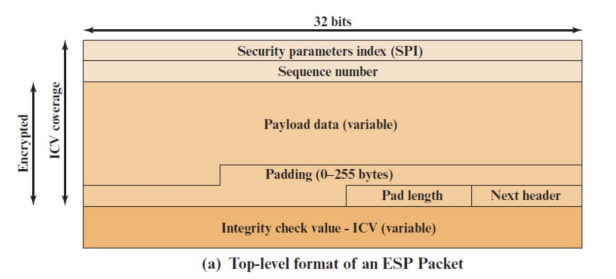
\includegraphics[width=1\textwidth]{images/chapter9/9-8.png}
    \caption{Reti wireless.}
    \label{fig:9-8}
\end{figure}

\begin{figure}[h]
    \centering
    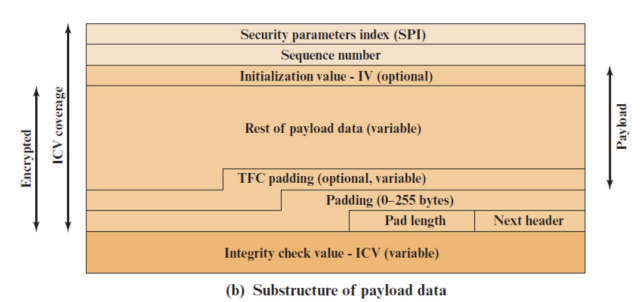
\includegraphics[width=1\textwidth]{images/chapter9/9-9.png}
    \caption{Reti wireless.}
    \label{fig:9-9}
\end{figure}

Nello specifico:
\begin{itemize}
    \item L'header specifica la crittografia e l'autenticazione. Quest'ultima è opzionale;
	\item Per la modalità di trasporto crittografa solo la parte di dati (carico utile) di ciascun pacchetto e lascia intoccato l'header;
	\item Per la modalità tunnel l'intero datagramma IP viene incapsulato all'interno dell'ESP. Il nuovo header può contenere indirizzi IP differenti (es: gateway di sicurezza). Il vecchio header e il payload vengono cifrati (e opzionalmente autenticati).
\end{itemize}

\section{Meccanismo per l'anti-replay}

Poiché la ricezione di pacchetti IP duplicati e autenticati può interrompere il servizio; il numero di sequenza viene usato per sviare questo tipo di attacchi:
\begin{itemize}
    \item Quando viene stabilito un nuovo SA, il mittente inizializza un contatore del numero di sequenza su 0, che viene incrementato ogni volta che un pacchetto viene inviato su questa SA;
	\item IP è senza connessione; non garantisce la consegna e la consegna in ordine;
	\item Il ricevitore implementa una finestra di dimensione W:
	\begin{itemize}
	    \item Se il pacchetto ricevuto cade nella finestra, viene controllato il MAC e se autenticato viene contrassegnato il suo slot ;
		\item Se il pacchetto ricevuto è sulla destra della finestra, vengono controllati MAC e auth e, se passati, la finestra viene spostata a destra;
		\item Se il pacchetto ricevuto è a sinistra o l'autenticazione non riesce, il pacchetto viene scartato.
	\end{itemize}
\end{itemize}

\begin{figure}[h]
    \centering
    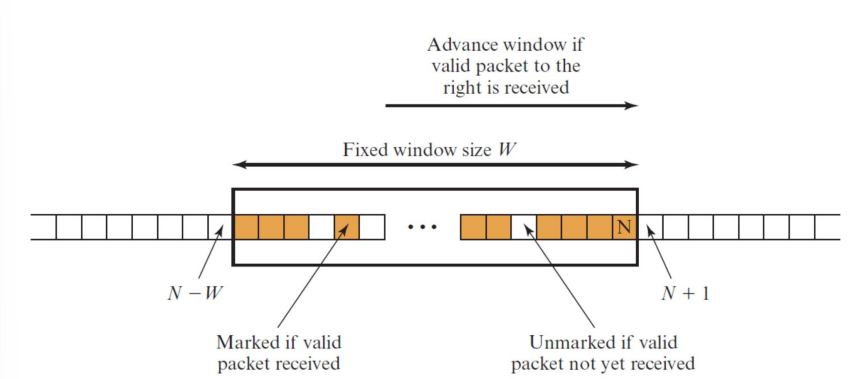
\includegraphics[width=1\textwidth]{images/chapter9/9-10.png}
    \caption{Reti wireless.}
    \label{fig:9-10}
\end{figure}

Modalità di trasporto per ESP

Funzionamemto:
	\item Alla fonte, il blocco di dati costituito dal trailer ESP più l'intero segmento del livello di trasporto viene crittografato e il testo in chiaro di questo blocco viene sostituito con il suo testo cifrato per formare il pacchetto IP per la trasmissione. L'autenticazione viene aggiunta se questa opzione è selezionata;
	\item Il pacchetto viene quindi instradato alla destinazione. Ogni router intermedio deve esaminare ed elaborare l'header IP più qualsiasi header di estensione IP in chiaro ma non ha bisogno di esaminare il testo cifrato;
	\item Il nodo di destinazione esamina ed elabora l'IP header più eventuali intestazioni di estensione IP in chiaro. Quindi, sulla base dell'SPI nell'intestazione ESP, il nodo di destinazione decrittografa il resto del pacchetto per recuperare il segmento del livello di trasporto in plain-text.
	
Il funzionamento in modalità trasporto garantisce la riservatezza per qualsiasi applicazione che lo utilizzi, evitando così la necessità di implementare la riservatezza in ogni singola applicazione. Uno svantaggio di questa modalità è che è possibile fare analisi del traffico  sui pacchetti trasmessi.

\subsection{Modalità tunnel}

La modalità Tunnel fornisce protezione al pacchetto IP:
\begin{enumerate}
    \item Per ottenere ciò, dopo aver aggiunto i campi AH o ESP al pacchetto IP, l'intero pacchetto più i campi di sicurezza vengono trattati come il payload del nuovo pacchetto IP esterno con un nuovo header IP esterno;
	2. L'intero pacchetto originale, ora interno, viaggia attraverso un tunnel da un punto all'altro di una rete IP; nessun router lungo il percorso è in grado di esaminare l'header IP interno;
	3. Poiché il pacchetto originale è incapsulato, il nuovo pacchetto più grande potrebbe avere indirizzi di origine e destinazione completamente diversi, aumentando la sicurezza;
\end{enumerate}

Caratteristiche:
\begin{itemize}
    \item La modalità Tunnel viene utilizzata quando una o entrambe le estremità della Security Association (SA) sono un gateway di sicurezza, come un firewall o un router che implementa IPsec;
	\item Con la modalità tunnel, gli host sulle reti dietro i firewall possono impegnarsi in comunicazioni sicure senza implementare Ipsec;
	\item I pacchetti non protetti generati da tali host vengono incanalati attraverso reti esterne tramite la modalità tunnel, come impostato dal software IPsec nel firewall o nel router sicuro al confine della rete locale.
	\item La modalità tunnel è utile in una configurazione che include un firewall o un altro tipo di gateway di sicurezza che protegge una rete affidabile da reti esterne;
	\item La crittografia avviene solo tra un host esterno e il gateway di sicurezza o tra due gateway di sicurezza:
	\begin{itemize}
	    \item Alleggerisce gli host sulla rete interna dall'elaborazione del carico di cifrare e semplifica l'attività di distribuzione delle chiavi riducendo il numero di chiavi necessarie;
		\item Contrasta l'analisi del traffico basata sulla destinazione finale.
	\end{itemize}
\end{itemize}

\section{Virtual Private Network (VPN)}

La modalità Tunnel può essere utilizzata per implementare una VPN. Una VPN è una rete privata configurata all'interno di una rete pubblica per sfruttare le economie di scala e le strutture di gestione delle grandi reti.

Vantaggi:
\begin{itemize}
    \item Le VPN sono ampiamente utilizzate dalle aziende per creare reti che si estendono su vaste aree geografiche, per fornire connessioni da sito a sito alle filiali e per consentire agli utenti mobili di collegarsi alle LAN aziendali;
	\item La struttura della rete pubblica è condivisa da molti clienti, con il traffico di ciascun cliente separato dall'altro traffico;
	\item Il traffico designato come traffico VPN può passare solo da una VPN sorgente verso una destinazione nella stessa VPN;
	\item Solitamente sono forniti crittografia e autenticazione per le VPN.
\end{itemize}

\begin{figure}[h]
    \centering
    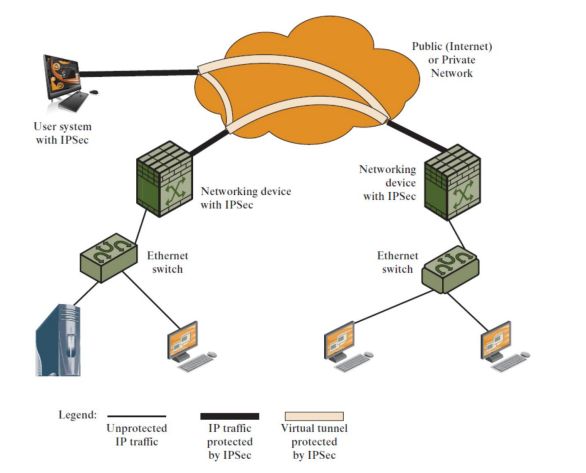
\includegraphics[width=1\textwidth]{images/chapter9/9-11.png}
    \caption{Reti wireless.}
    \label{fig:9-11}
\end{figure}

\section{Riassunto}

\begin{table}[h]
    \centering
    \begin{tabular}{ |p{0.5\textwidth}|p{0.5\textwidth}|p{0.5\textwidth}| }
         \hline
          & Modalità di trasporto SA & Modalità tunnel SA \\ 
         AH & Autentica il payload IP e porzioni selezionate dell'intestazione IP e delle intestazioni dell'estensione IPv6. & Autentica l'intero pacchetto IP interno (header interno più payload IP) più porzioni selezionate dell'header esterno IP e dell'estensione esterna di IPv6 \\ 
         ESP & Crittografa il payload IP e qualsiasi header di estensione IPv6 che segue l'header ESP. & Crittografa l'intero pacchetto IP interno. \\ 
         ESP con autenticazione & Crittografa il payload IP e qualsiasi intestazione di estensione IPv6 dopo l'header ESP. Autentica il payload IP ma non l'header IP.& Crittografa l'intero pacchetto IP interno. Autentica il pacchetto IP interno. \\ 
         \hline
    \end{tabular}
    \caption{Riassunto.}
    \label{tab:table9-1}
\end{table}

\section{Internet Key Exchange}

La parte di gestione chiave di IPsec comporta la determinazione e distribuzione delle chiavi segrete. Un requisito tipico sono quattro chiavi per la comunicazione tra due applicazioni (una coppià per integrità e una per crittografia/riservatezza).

Il documento IPsec Architecture richiede il supporto per due tipi di gestione delle chiavi:
\begin{itemize}
    \item Manuale: un amministratore di sistema configura manualmente ogni sistema con le proprie chiavi e con le chiavi di altri sistemi comunicanti (pratico per ambienti piccoli e statici);
	\item Automatizzato: consente la creazione on-demand di chiavi per SA e facilita l'utilizzo delle chiavi in un grande sistema distribuito con una configurazione in evoluzione.
\end{itemize}

\subsection{Overview}

\begin{figure}[h]
    \centering
    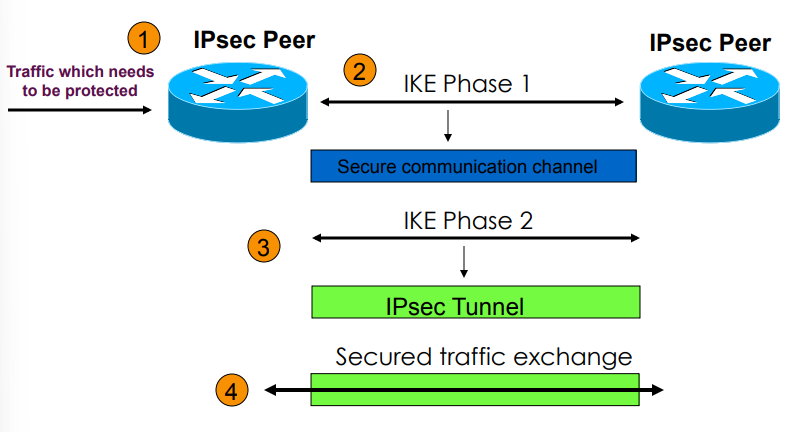
\includegraphics[width=1\textwidth]{images/chapter9/9-12.png}
    \caption{Reti wireless.}
    \label{fig:9-12}
\end{figure}

La creazione del canale può avvenire in due modi:
\begin{itemize}
    \item Main mode: i due peer non si conoscono e devono creare una canale sicuro di comunicazione. Una volta stabiliti i segreti e creato il canale, questo può essere usato epr scambiarsi altri segreti e creare sottocanali;
	\item Quick mode: usata per creare canali figli. 
\end{itemize}

Se un canale main o figlio viene compromesso, gli altri sono comunque sicuri.

\subsection{Main mode/Fase 1}

\begin{figure}[h]
    \centering
    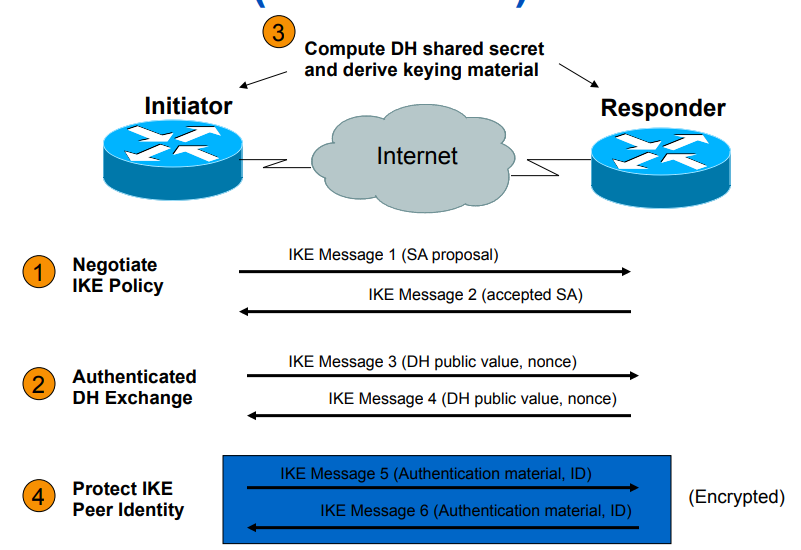
\includegraphics[width=1\textwidth]{images/chapter9/9-13.png}
    \caption{Reti wireless.}
    \label{fig:9-13}
\end{figure}

Vengono scambiati sei messaggi, a coppie di due:
\begin{enumerate}
    \item L'initiator invia una serie di proposte e un elenco di algoritmi per ogni per ogni proposta. Il responder risponde con le proposte accettate e l'algoritmo scelto per ogni proposta;
	\item Scambio autenticato delle mezze chiavi di DH e dei nonce;
	\item Scambio dell'hash crittografato della propria identità e dei messaggi scambiati, con seguente confronto.
\end{enumerate}

\subsection{ISAKMP/Oakley}

Protocollo di gestione delle chiavi automatizzato predefinito di Ipsec.

Si compone di:
\begin{itemize}
    \item  Oakley Key Determination Protocol:
	\begin{itemize}
	    \item Protocollo di scambio di chiavi basato sull'algoritmo Diffie-Hellman ma che fornisce una maggiore sicurezza;
		\item Generico in quanto non detta formati specifici
	\end{itemize}
	\item Internet Security Association and Key Management Protocol (ISAKMP):
	\begin{itemize}
	    \item Fornisce un framework per la gestione delle chiavi Internet e fornisce il supporto per il  protocollo specifico, inclusi i formati, per la negoziazione degli attributi di sicurezza;
		\item Consiste in un insieme di tipi di messaggi che consentono l'uso di una varietà di algoritmi di scambio di chiavi.
	\end{itemize}
\end{itemize}

IKE è caratterizzato da cinque caratteristiche importanti:
\begin{itemize}
    \item Impiega un meccanismo noto come cookie per contrastare attacchi di intasamento;
	\item Consente alle due parti di negoziare un gruppo; questo, in sostanza, specifica i parametri globali dello scambio di chiavi Diffie-Hellman;
	\item Usa i nonce per proteggersi dai replay attack;
	\item Consente lo scambio delle chiavi pubbliche di DF;
	\item Autentica lo scambio Diffie-Hellman per contrastare gli attacchi man-in-the-middle.
\end{itemize}

\begin{figure}[h]
    \centering
    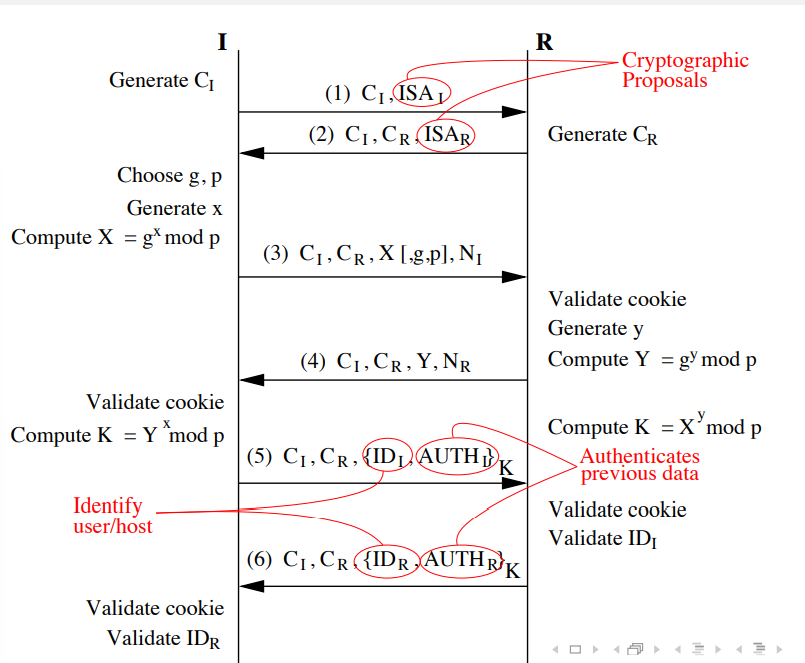
\includegraphics[width=1\textwidth]{images/chapter9/9-14.png}
    \caption{Reti wireless.}
    \label{fig:9-14}
\end{figure}

Quick mode/Fase 2

Tutto il traffico è cifrato usando ISAKMP Security Association. Ciascuna negoziazione in modalità rapida risulta in due IPsec Security Association, una in entrata e una in uscita. Vengono create/aggiornate le chiavi necessarie. 
Si può fare subito il DF autenticato facendo viaggiare il messaggio con un hash storico (il secondo messaggio viaggia con l'hash del primo e del secondo) generato dalla Master Key scambiata nella fase 1. Nei nuovi canali è possibile cambiare i parametri.

\begin{figure}[h]
    \centering
    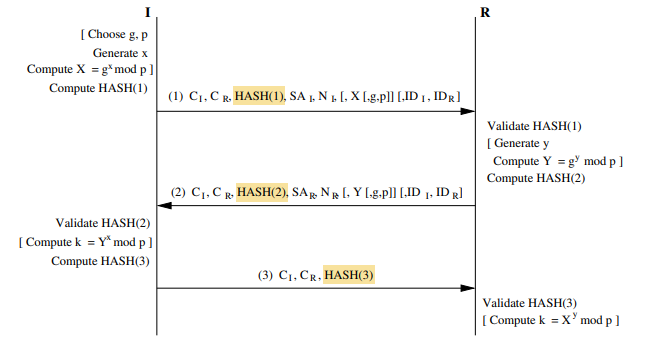
\includegraphics[width=1\textwidth]{images/chapter9/9-15.png}
    \caption{Reti wireless.}
    \label{fig:9-15}
\end{figure}

\begin{figure}[h]
    \centering
    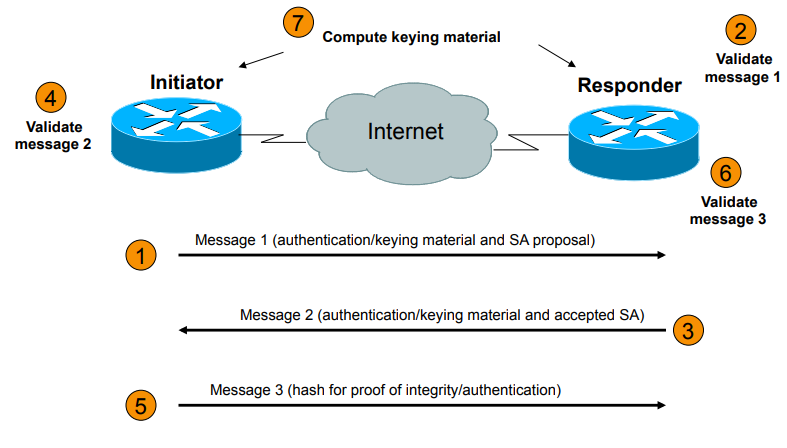
\includegraphics[width=1\textwidth]{images/chapter9/9-16.png}
    \caption{Reti wireless.}
    \label{fig:9-16}
\end{figure}

\section{Combinazione di associazioni di sicurezza }

Una singola SA può implementare il protocollo AH o ESP, ma non entramb.

Security Association bundle:
\begin{itemize}
    \item Si riferisce a una sequenza di SA attraverso le quali deve essere elaborato il traffico per fornire l'insieme di servizi IPsec desiderato;
	\item Le SA in un bundle possono terminare a diversi endpoint o allo stesso punto finale.
\end{itemize}

I bundle possono essere creati in due modi:
\begin{itemize}
    \item Adiacenze di trasporto:
	\begin{itemize}
	    \item Si riferisce all'applicazione di più di un protocollo di sicurezza allo stesso pacchetto IP senza invocare il tunneling;
		\item Questo approccio consente un solo livello di combinazione;
	\end{itemize}
	\item Tunneling iterato:
	\begin{itemize}
	    \item Si riferisce all'applicazione di più livelli di protocolli di sicurezza effettuati tramite il tunneling IP;
		\item Questo approccio consente più livelli di nidificazione.
	\end{itemize}
\end{itemize}

\section{ESP con opzione di autenticazione}

In questo approccio, il primo utente applica ESP ai dati da proteggere e poi aggiunge il campo di autenticazione dei dati. 

Varia in base alla modalità:
\begin{itemize}
    \item Modalità di trasporto ESP: l'autenticazione e la crittografia si applicano al payload IP consegnato all'host, ma l'intestazione IP non è protetta;
	\item Modalità tunnel ESP: l'autenticazione si applica all'intero pacchetto IP consegnato all'indirizzo IP di destinazione esterno e l'autenticazione viene eseguita a quella destinazione. L'intero pacchetto IP interno è protetto dal meccanismo di privacy per la consegna alla destinazione IP interna.
\end{itemize}

In entrambi i casi l'autenticazione si applica al testo cifrato anziché al testo in chiaro.

\section{Adiacenze dei trasporti}

Un altro modo per applicare l'autenticazione dopo la crittografia consiste nell'usare due SA di trasporto in bundle, con all'interno un ESP SA e all'esterno un AH SA:
\begin{itemize}
    \item In questo caso l'ESP viene utilizzato senza la sua opzione di autenticazione;
	\item La crittografia viene applicata al payload IP;
	\item AH viene quindi applicato in modalità di trasporto;
	\item Il vantaggio di questo approccio è che l'autenticazione copre più campi;
	\item Lo svantaggio è l'overhead di due SA contro una SA.
\end{itemize}

\section{Transport-Tunnel Bundle}

L'uso dell'autenticazione prima della crittografia potrebbe essere preferibile per diversi motivi:
\begin{itemize}
    \item È impossibile per chiunque intercettare il messaggio e alterare i dati di autenticazione senza essere scoperti;
	\item Potrebbe essere opportuno memorizzare le informazioni di autenticazione con il messaggio alla destinazione per riferimenti futuri.
\end{itemize}

Un approccio consiste nell'utilizzare un bundle costituito da un trasporto AH interno SA e un tunnel ESP esterno SA:
\begin{itemize}
    \item L'autenticazione viene applicata al payload IP e all'header IP;
	\item Il pacchetto IP risultante viene quindi elaborato in modalità tunnel da ESP;
	\item Il risultato è che l'intero pacchetto interno autenticato viene crittografato e viene aggiunta una nuova intestazione IP esterna.
\end{itemize}







\setchapterpreamble[u]{\margintoc}
\chapter{Reti anonime}
\labch{chapter10}

Privacy sulle reti pubbliche:
\begin{itemize}
    \item Internet è disegnato come una rete pubblica: le macchine potrebbero vedere il traffico delle altre e i router vedono tutto il traffico che passa loro attraverso;
	\item Le info dul routing sono pubbliche: è facile capire chi sta comunicando con chi osservando l'header IP;
	\item La crittografia non nasconde le identità: la crittografia nasconde il payload, ma non il routing. Anche IPsec (tunnel mode/ESP) rivela gli indirizzi IP al gateway IPsec.
\end{itemize}

Applicazioni dell'anonimità:
\begin{itemize}
    \item Privacy;
	\item Email irrintracciabili;
	\item  Comunicazioni segrete su reti pubbliche;
	\item Denaro digitale (acquisti online non linkabili all'identità del compratore);
	\item Voto elettronico anonimo;
	\item Pubblicazioni contro la censura.
\end{itemize}
	
Cos'è l'anonimità:
\begin{itemize}
    \item Stato in cui non si è identificabile all'interno di un insieme di soggetti (nascono le mie attività tra altri simile; non posso essere anonimo da solo);
	\item Incollegabilità tra azione e identità;
	\item Inosservabilità (l'osservatore non riesce a dire se l'azione è stata fatta o no, difficile da ottenere).
\end{itemize}

Attacchi all'anonimità:
\begin{itemize}
    \item Analisi passiva del traffico: cerco di capire dal traffico della rete chi parla con chi;
	\item Analisi del traffico attiva: inietto pacchetti;
	\item Compromissione dei nodi della rete (router): non è ovvio capire quale nodo è stata compromesso.
\end{itemize}

L'anonimato è il migliore quando il servizio di anonimizzazione attira molti utenti (TOR).



%----------------------------------------------------------------------------------------
\end{document}
